\documentclass{bcc}
\usepackage{amssymb}
\usepackage{fancyhdr}


%Para aparecer XML como codigo
\usepackage{listings}
\usepackage{color}
\usepackage{comment}
\usepackage{url}
%\definecolor{codegreen}{rgb}{0,0.6,0}
%\definecolor{codegray}{rgb}{0.5,0.5,0.5}
%\definecolor{codepurple}{rgb}{0.58,0,0.82}
%\definecolor{backcolour}{rgb}{0.95,0.95,0.92}
%\lstdefinestyle{mystyle}{
%    backgroundcolor=\color{backcolour},   
%    commentstyle=\color{codegreen},
%    keywordstyle=\color{magenta},
%    numberstyle=\tiny\color{codegray},
%    stringstyle=\color{codepurple},
%    basicstyle=\footnotesize,
%    breakatwhitespace=false,         
%    breaklines=true,                 
%    captionpos=b,                    
%    keepspaces=true,                 
%    numbers=left,                    
%    numbersep=5pt,                  
%    showspaces=false,                
%    showstringspaces=false,
%    showtabs=false,                  
%    tabsize=2
%}
%\lstset{style=mystyle}

\definecolor{maroon}{rgb}{0.5,0,0}
\definecolor{darkgreen}{rgb}{0,0.5,0}
\lstdefinelanguage{xml}
{
  basicstyle=\ttfamily,
  morestring=[s]{"}{"},
  morecomment=[s]{?}{?},
  morecomment=[s]{!--}{--},
  commentstyle=\color{darkgreen},
  moredelim=[s][\color{black}]{>}{<},
  moredelim=[s][\color{red}]{\ }{=},
  stringstyle=\color{blue},
  identifierstyle=\color{maroon},
  basicstyle=\footnotesize,
  breakatwhitespace=false,         
  breaklines=true,                 
  captionpos=b,                    
  keepspaces=true,                 
  numbers=left,                    
  numbersep=5pt,                  
  showspaces=false,                
  showstringspaces=false,
  showtabs=false,                  
  tabsize=2
}

\lstdefinelanguage{txt}
{
  basicstyle=\ttfamily,
  basicstyle=\footnotesize,
  breakatwhitespace=true,         
  breaklines=true,                 
  captionpos=b,                    
  keepspaces=false,                 
  numbers=none,                    
  numbersep=5pt,                  
  showspaces=false,                
  showstringspaces=false,
  showtabs=false,                  
  tabsize=2
}
%Para aparecer XML como codigo


\titulo{OrCA: uma Ferramenta Baseada em Linguagem Natural Controlada para Construção Automática de Ontologias}
\palavrasChave{Ontologias}{Processamento de Linguagem Natural}{Raciocínio Automático.  Representação de Conhecimento}
\keywords{Ontologies. Natural Language Processing. Automatic Reasoning. Knowledge Representation.}

\autor{Paulo Mateus da Silva}{paulomatew@gmail.com}

\orientador{Ryan Azevedo}{UAG - UFRPE}{}
%\orientadorDois{John von Neumann}{UAG}{UFRPE}
% \orientadorTres*{Ada Lovelace}{UAG}{UFRPE} % Se feminino use *, tanto para orientador ou examinador

\examinador{Assuero Ximenes Fonseca}{UAG - UFRPE}{}
\examinadorDois{Levy Souza Silva}{UNINASSAU - Caruaru/PE}{}
%\examinadorTres{Stephen Cook}{UAG}{UFRPE}
%\examinadorQuatro{John Backus}{UAG}{UFRPE}

\dataMesAno{04}{julho}{2019}

\begin{document}

\selectlanguage{portuguese}

\capa

% \capaDois
\begin{agradecimentos}
AGRADECIMENTOS
\end{agradecimentos}


\begin{resumo}

Com a crescente necessidade de capturar, representar e compartilhar conhecimento entre humanos e máquinas, desenvolvemos a ferramenta OrCA. Uma ferramenta para construção automática de ontologias baseada em Processamento de Linguagem Natural, cujo objetivo é o de criar de forma semiautomática, com pouca ou nenhuma intervenção humana, ontologias expressivas em OWL DL. A ferramenta também é capaz  de realizar raciocínio automático de inconsistências e subsunção em tempo de desenvolvimento. Ontologias são especificações formais e compartilhadas de um domínio de conhecimento. Para uma maior adoção do uso e do desenvolvimento de ontologias, tanto por parte de profissionais experientes como leigos interessados em seu desenvolvimento faz-se-a necessário a criação de ferramentas que facilitem esse processo. Com isto, permitindo que usuários com pouco conhecimento em Web Semântica ou em desenvolvimento de ontologias possam se engajar no desenvolvimento de ontologias modeladas em OWL DL. Nossos resultados demostram o sucesso do OrCA em criar ontologias com baixo ou alto nível de complexidade baseada numa Linguagem Natural Controlada e com capacidade de realizar raciocínio automático.

\end{resumo}

\selectlanguage{english}

\begin{abstract}
Due to the growing need to capture, represent and share knowledge between humans and machines, we developed the OrCA tool. A tool for automatic ontology construction based on Natural Language Processing, whose goal is to create semi-automatic expressive ontologies in OWL DL, with little or no human intervention. Also, the tool is capable of performing automatic reasoning of inconsistencies and subsumption at execution time. Ontologies are formal and shared specifications of a knowledge domain. In order to disseminate and develop the ontologies usage, not only for experienced professionals, but also for laypeople interested in, it will be necessary to create tools that facilitate this process. Through such tools, people with little knowledge either in Semantic Web or Ontologies can be engaged in the development of Ontologies modeled in OWL DL. Our results demonstrate the success of OrCA by creating Ontologies with low or high level of complexity based on a Controlled Natural Language and with the ability to perform automatic reasoning.

\end{abstract}


\selectlanguage{portuguese}

% Centralizar titulos
\renewcommand\contentsname{\centerline{Sumário}}
\renewcommand\listfigurename{\centerline{Lista de Figuras}}
\renewcommand\listtablename{\centerline{Lista de Tabelas}}

\lhead{Sumário}
\tableofcontents

\listoffigures
\addcontentsline{toc}{chapter}{Lista de Figuras}

\listoftables
\addcontentsline{toc}{chapter}{Lista de Tabelas}

\inicio
\chapter{Introdução}

A razão pela qual ontologias estão se tornando tão populares é em grande parte devido ao que elas prometem: um entendimento comum e compartilhado de alguns domínios de conhecimento que podem ser utilizados entre pessoas e sistemas \cite{fensel2001}. Além disso, são consideradas artefatos essenciais em muitas aplicações.

Sistemas que processam linguagem natural (ou de Processamento de Linguagem Natural, PLN) têm o intuito de converter a linguagem usada por humanos em uma representação formal para que computadores entendam, manipulem e troquem informações com usuários, para isso, faz-se necessário a integração de diversas áreas do conhecimento como Processamento de Linguagem Natural \cite{brill1995}, Representação de Conhecimento \cite{levesque1986} e Raciocínio Automático \cite{wos1984}.

Com a utilização do PLN é possível descobrir verbos, sujeitos, sinônimos e até mesmo identificar conceitos (desde que o sistema possua um vocabulário controlado) em um texto. Mas para tarefas mais complexas, faz-se-a necessário a utilização de ontologias. Ontologias podem ser usadas para inferências complexas e derivação de regras necessárias para a interpretação semântica e sistemas de perguntas e respostas. Por essa razão, as ontologias têm sido de particular interesse para pesquisadores que desenvolvem sistemas inteligentes \cite{liu2011}.

O termo ontologia existe em diversas áreas, em computação o termo recebe a seguinte definição: uma ontologia é uma especificação formal e explícita de uma conceituação compartilhada \cite{gruber1995}.

Ontologias são componentes importantes em Sistemas de Informação \cite{estival2004}. Por isso, nem todos os desenvolvedores de ontologias são programadores ou de áreas correlatas a Tecnologia da Informação e Comunicação. Portanto, a criação de \textit{softwares} capazes de criar ontologias e mitigar a dificuldade de sua construção, possibilitando que profissionais interessados em seu desenvolvimento é de bastante relevância para assim poderem desenvolver suas bases de conhecimento modeladas como ontologias. Existem muitas ferramentas que são capazes de criar ontologias, entre elas \textit{Protégé} \cite{noy2001} e \textit{yEd Graph Editor}. Porém devido a quantidade de plugins e recursos disponíveis dentro dessas ferramentas, pode acabar dificultando o processo de desenvolvimento dos usuários.

A ferramenta OrCA (\textit{Ontology vieweR and CreAtor}) surgiu com o objetivo de ser um sistema computacional baseado em linguagem natural controlada para criação de ontologias. Embora o \textit{Protégé} possua diversos recursos, funções e plugins, a OrCA tem como objetivo ser uma versão objetiva e mais "\textit{clean}", englobando as funções necessárias no desenvolvimento de ontologias, permitindo ao usuário a criação e visualização de ontologias (textual e gráfica), de maneira simples e rápida.

%Os desenvolvedores de ontologias geralmente capturam os relacionamentos entre entidades como relacionamentos formais e lógicos. Para fazer isso, geralmente se utiliza a lógica descritiva \cite{liu2011}.

\section{Definição do Problema}

Atualmente, o processo de desenvolvimento de ontologias é em grande parte manual, mesmo usando ferramentas e processos de desenvolvimento. Os usuários devem adicionar conceitos e relacionamentos, um por um. O investimento no desenvolvimento de ontologias é imenso \cite{liu2011}. Surge então a necessidade e a importância de facilitar e viabilizar esse desenvolvimento para que usuários com diversos níveis de conhecimento e experiência possam participar ativamente do processo de desenvolvimento.

Existem muitas ferramentas de construção de ontologias que podem ser usadas, mas há algumas dificuldades para o especialista em domínio entender o significado entre essas abordagens, como a abordagem de geração pouco clara, a linguagem de ontologia não unificada e assim por diante, tais questões tornam grande a curva de aprendizado para utilização dessas ferramentas \cite{zhou2010}. Um exemplo dessas ferramentas é o \textit{Protégé}, que é uma ferramenta de autoria de ontologias, porém, como muitas outras ferramentas similares, ela exige habilidades especializadas em engenharia de ontologia \cite{funk2007}. Além destas habilidades, muitas vezes é requerido um alto nível de conhecimento na área de Web Semântica e também de tempo e esforço para aprender a usá-las, devido a quantidade de recursos e funcionalidades.

Diante deste contexto, surge a necessidade de uma ferramenta que tenha o objetivo de facilitar e viabilizar o processo de desenvolvimento de ontologias, permitindo que esse processo seja mais simples, e não exija do usuário conhecimento prévio de linguagem de programação ou Web Semântica e que não seja muito complexa em seu uso, tornando maior o número de usuários que poderão participar ativamente da criação de ontologias.

\section{Trabalhos Relacionados}

Alguns trabalhos similares foram encontrados, como o sistema apresentado em \cite{mousavi2013} que é baseado em PLN, chamado OntoHarvester; um gerador de ontologias distribuído (utilizando os serviços da Amazon EC2 e S3) e não supervisionado, que gera automaticamente ontologias de um domínio a partir de texto não estruturado. Como a definição mostra, tem como objetivo grandes blocos de textos como entrada, assim como gerar grandes ontologias como saída, que difere do objetivo da OrCA. 

No trabalho feito em \cite{wachter2011} os autores apresentam o DOG4DAG que é uma ferramenta de geração de ontologias no OBO-edit \cite{day2007} que visa facilitar o trabalho dos engenheiros de ontologia, que criam ontologias a partir do zero ou estendem as ontologias existentes. Porém o objetivo apresentado é o de facilitar o processo de desenvolvimento para usuário que já trabalham e possuem conhecimento de ontologias, diferentemente da solução adotada pela OrCA, o DOG4DAG não isenta o usuários de conhecimentos mais profundos.

Em \cite{zhou2010} é exibido o trabalho que desenvolveu uma ferramenta geradora de ontologia que é implementada com base no Jena na plataforma Java, a ferramenta tem o objetivo de fornecer ontologia unificada e melhorar a qualidade da ontologia e gerar de ontologias a partir de banco de dados relacional (RDB2On) baseado em Jena\cite{jena}. A ferramenta, apesar de facilitar e fornecer uma abordagem diferente para a geração de ontologias, ainda requer do usuário conhecimento técnico.

Através dos resultados obtidos nos testes realizados com a ferramenta desenvolvida, foi possível observar seu sucesso em gerar códigos OWL que representam ontologias, recebendo como entrada textos em linguagem natural. O uso de linguagem natural facilita a usabilidade, diminuindo a curva de aprendizagem, uma vez que o utilizador não precisa ter conhecimento em linguagens de programação, web semântica ou engenharia de ontologias, apenas conhecimento das palavras reservadas pelo compilador e como usá-las.


\section{Objetivos}

A seguir são descritos os objetivos gerais e específicos que foram definidos e que este trabalho deseja atingir.

\section{Objetivo Geral}
O objetivo geral deste trabalho foi desenvolver uma ferramenta computacional baseada em Processamento de Linguagem Natural para construção automática de Ontologias a partir de texto (Linguagem Natural Controlada). A esse objetivo Geral apresentamos os seguintes objetivos específicos.

\subsection{Objetivos Específicos}
•	Desenvolvimento de uma Linguagem Natural Controlada para criação de código OWL DL;

•	Construir ontologias em OWL DL com expressividade de alto nível (mínima ALC);

•	Apoiar engenheiros e desenvolvedores no processo de construção de bases de conhecimento modeladas como ontologias;

•	Permitir que usuários acelerem o desenvolvimento das bases de conhecimento modeladas como ontologias no qual são gerados automaticamente códigos OWL DL a partir dos textos inseridos;

•	Construir uma ferramenta capaz de realizar raciocínio de subsunção deduzindo que classes são subclasses de outras, a partir de suas respectivas descrições;

•	Detectar e verificar inconsistências em tempo de desenvolvimento nas ontologias construídas.

\section{Organização do Texto}

Além deste capítulo inicial que traz uma introdução sobre o tema, a motivação e justificativa para realização do trabalho, a definição do problema e o objetivo; este trabalho está organizado em mais 4 capítulos, como seguem:

• O \autoref{chap:fundamentacao} apresenta a fundamentação teórica, contendo referências bibliográficas de estudos na área e das ferramentas e conceitos que foram utilizados no desenvolvimento da ferramenta;

• O \autoref{chap:sistema} mostra a arquitetura do sistema, seus componentes, funcionamento e a maneira que ele foi desenvolvido;

• O \autoref{chap:exp} expõe os experimentos que foram realizados para validar a ferramenta, assim como seus respectivos resultados.


\chapter{Fundamentação teórica}
\label{chap:fundamentacao}

Nesta seção são apresentados os conceitos e ferramentas que foram utilizados no desenvolvimento deste projeto e as respectivas justificativas que embasam o uso de cada um deles.

\section{Ontologia}

Existem diversas técnicas que podem ser utilizadas para organizar informações e conhecimento, a aplicação de ontologias tem recebido uma atenção cada vez maior \cite{almeida2014}. O termo pode ser encontrado não apenas na ciência da computação, mas também em diversas áreas do conhecimento, por isso, é importante entender seu significado e sua aplicação em cada área específica.

O termo ontologia teve origem no século XVII na área da filosofia, a palavra vem do grego e pode ser traduzida como estudo da existência \cite{guizzardi2005}. Segundo \cite{gruber1995} o termo é emprestado da filosofia onde uma Ontologia é uma explicação sistemática da existência. Para um sistema de Inteligência Artificial, o que existe é tudo aquilo que pode ser representado.

Na computação, o termo foi usado pela primeira vez no fim dos anos 70 e desde então, ontologias têm sido aplicadas em uma infinidade de áreas da ciência da computação, uma das motivações foi a necessidade de criar representações de princípios de conhecimento de domínio na comunidade de compartilhamento e reutilização de conhecimento em IA \cite{guizzardi2005}.

Em áreas relacionadas com Modelagem Conceitual, ontologias são usadas de acordo com dua definição em Filosofia. Na Inteligência Artificial, Engenharia de Software e \textit{Web} Semântica geralmente ontologia é usada como: (i)um artefato concreto de engenharia desenhado com um intuito específico sem focar muito em questões de fundamentação ou (ii) uma representação de um domínio particular que pode ser expressa em alguma linguagem de representação de conhecimento (RDF, OWL, F-Logic) ou de modelagem conceitual (UML, EER) \cite{guizzardi2008}. Neste trabalho, será considerada a definição ii, que é a mais utilizada na área de Inteligência Artificial.

Segundo \cite{gruber1995} uma ontologia é uma especificação formal e explícita de uma conceituação compartilhada. A partir da definição dada por Gruber, \cite{rocha2014} complementa o pensamento afirmando que “formal”, significa que é definido declarativamente para que possa ser compreendido por agentes inteligentes; “explícito”, significa que os elementos e suas restrições estão claramente definidos; “conceituação”, representa um modelo abstrato de um campo de conhecimento ou um universo limitado de discurso; “compartilhado”, indica que é um conhecimento consensual, uma terminologia comum do campo modelado \cite{rocha2014}.

\cite{lv2011} afirma que o principal papel das ontologias é melhorar a comunicação entre humanos ou entre computadores, especificando a semântica do aparato simbólico usado no processo de comunicação.

Ontologias podem ser representadas de maneira formal, usada para que elas possam ser processada por comutadores, ou de maneira gráfica, usada para facilitar a compreensão humana \cite{isotani2015}. As linguagens mais populares para descrever ontologias são RDF, RDF-S e OWL \cite{mcguinness}.


\section{OWL}

A web atual possui deficiências que serão superadas com o uso da Web Semântica. Portanto, se faz necessária uma linguagem para descrever as ontologias que permitem a Web Semântica. A\textit{Web Ontology Language} (OWL) OWL é uma linguagem para definir ontologias e dados individuais associados. Sistemas de raciocínio baseados em quadros, lógicas de descrição e linguagens da Web existentes influenciaram o desenvolvimento da OWL, que foi desenvolvida para representar informações analisáveis por computador \cite{lacy2005}.

A OWL é projetada para ser usada por aplicações que precisam processar o conteúdo da informação em vez de apenas apresentar informações aos seres humanos. OWL fornece uma maior facilidade para a máquina interpretar o conteúdo da Web do que linguagens suportadas por XML, RDF e RDF Schema (RDF-S), pois fornece vocabulário adicional junto com uma semântica formal. Ela possui três sub-linguagens cada vez mais expressivas: OWL Lite, OWL DL e OWL Full \cite{mcguinness}. Na Figura \ref{fig:owlsub} é possível observar uma pequena definição sobre cada uma dessas sub-linguagens de OWL.

\begin{figure}[H]
\centering
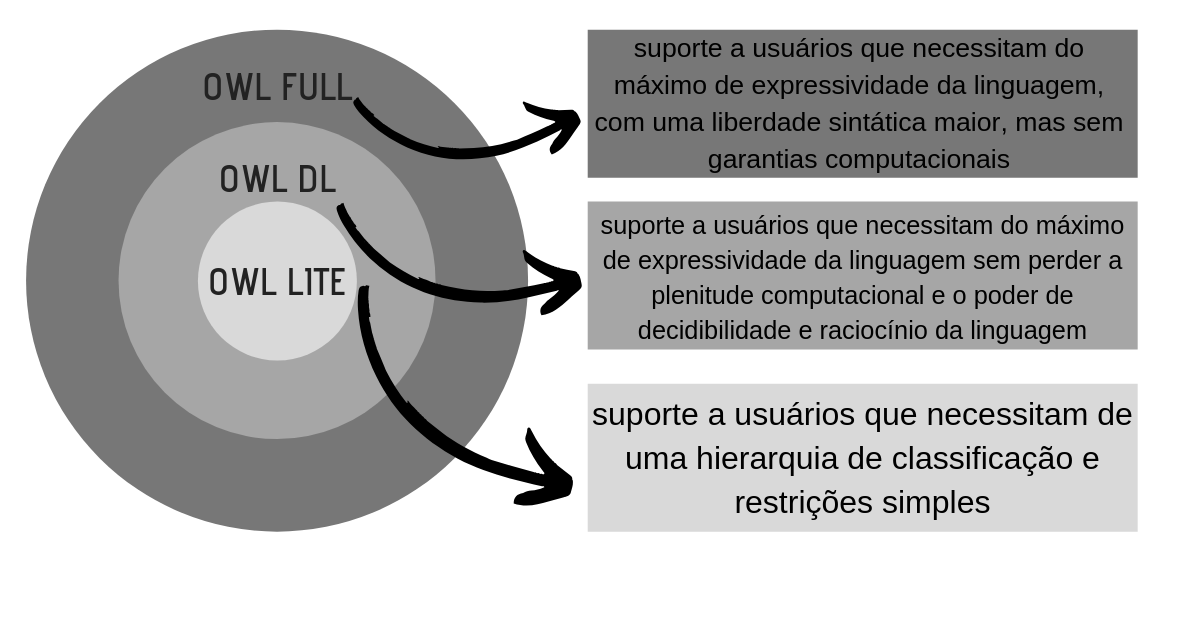
\includegraphics[width=.9\textwidth]{Figuras/owl_sub.png}
\caption{Sub-linguagens de OWL}
\label{fig:owlsub}
\end{figure}

Através da definição do conceito de bicicleta, é possível ter um exemplo de uma representação formal: uma bicicleta (\textit{bicycle}) é um tipo de veículo (\textit{vehicle}) de transporte, ou seja, pode ser feita a relação “\textit{bicycle is-a vehicle}”. Além disso, um bicicleta pode ser categorizada em bicicletas esportivas (\textit{sport bicycle}) e bicicletas para uso na cidade (\textit{city bicycle}). Por fim, é possível identificar os atributos e propriedades da bicicleta como cor, peso, tamanho, etc. O resultado disto, pode ser visto na Figura \ref{fig:codowl}, onde se encontra parte do código de uma ontologia em OWL que descreve uma bicicleta \cite{isotani2015}.


\begin{figure}[H]
\centering
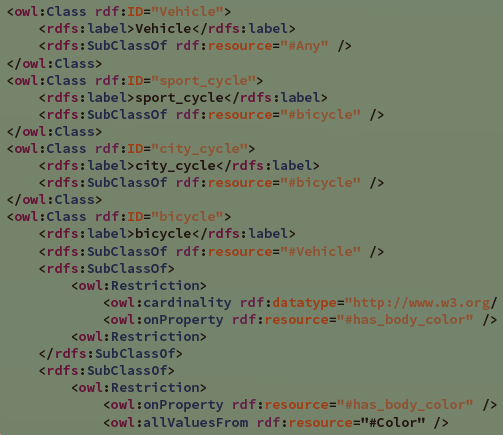
\includegraphics[width=.9\textwidth]{Figuras/codigo_owl.png}
\caption{Exemplo de código OWL. Fonte: http://hozo.jp/}
\label{fig:codowl}
\end{figure}

\subsection{Elementos básicos}
 
Para construir uma ontologia OWL, são necessários alguns elementos básicos, são eles as classes, instâncias das classes (indivíduos) e os relacionamentos entre instâncias (propriedades).
 
Classes fornecem um mecanismo de abstração para agrupar recursos com características semelhantes. Cada classe OWL é associada a um conjunto de indivíduos, chamado de extensão de classe. Os indivíduos na extensão de classe são chamados de instâncias da classe \cite{mcguinness}. 

Cada indivíduo na OWL é membro da classe \textit{owl:Thing}. Assim, ela é superclasse de todas as classes OWL definidas pelos usuários. Além disso, existe a classe \textit{owl:Nothing} (não possui instâncias) que é uma subclasse de todas as classes OWL. Uma classe é sintaticamente representada como uma instância nomeada da \textit{owl:Class} \cite{de2005}.

Uma propriedade é uma relação binária que pode ser de dois tipos:

• Propriedades de dados tipados: relação entre indivíduos e valores
de dados;

• Propriedades de objetos: relação entre indivíduos \cite{welty2004}.

\subsubsection{Restrições em propriedade}

OWL permite que sejam impostas restrições sobre propriedades, restrição é um tipo especial de descrição de classe, isto é, descreve uma classe anônima de indivíduos que satisfazem as restrições \cite{de2005}.

A restrição \textit{allValuesFrom} e a \textit{someValuesFrom} são exemplos de restrição de valores. A \textit{owl:allValuesFrom} é usada para descrever uma classe de todos os indivíduos para os quais todos os valores da propriedade em questão são membros da extensão de classe da descrição da classe ou são valores de dados dentro do intervalo de dados especificado \cite{welty2004}, um exemplo do uso dessa propriedade por ser observado na Figura \ref{fig:allvalues}.

\begin{figure}[H]
\centering
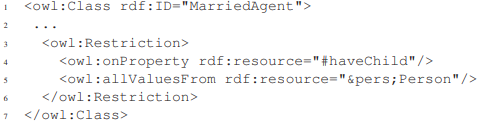
\includegraphics[width=.9\textwidth]{Figuras/all_values.PNG}
\caption{Exemplo de uso da restrição allValuesFrom}
\label{fig:allvalues}
\end{figure}

A restrição \textit{someValuesFrom} descreve uma classe de todos os indivíduos para os quais pelo menos um valor da propriedade em questão é uma instância da descrição da classe ou um valor de dados no intervalo de dados \cite{welty2004}. Um exemplo do uso dessa propriedade por ser visto na Figura \ref{fig:somevalues}.

\begin{figure}[H]
\centering
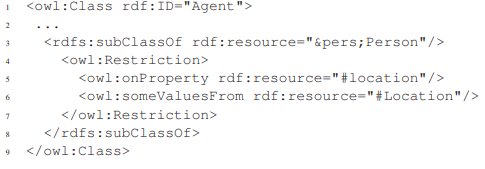
\includegraphics[width=.9\textwidth]{Figuras/some_values.PNG}
\caption{Exemplo de uso da restrição someValuesFrom}
\label{fig:somevalues}
\end{figure}

\subsection{Conjunto de Operadores}

OWL permite combinações booleanas arbitrárias para manipulações das extensões de classes, chamados de conjunto de operadores, eles podem ser vistos como representando os operadores AND, OR e NOT nas classes. Os três operadores obtêm os nomes padrão de operador de conjunto: interseção, união e complemento \cite{bechhofer2004}.

• \textit{owl:intersectionOf}: semelhante ao operador lógico AND, declara uma classe cuja extensão de classe contém somente indivíduos que são membros da extensão de classe de todas classes descritas em uma lista \cite{bechhofer2004}. Um exemplo de um trecho de código que utiliza este operador pode ser encontrado na Figura \ref{fig:opand}.

\begin{figure}[H]
\centering
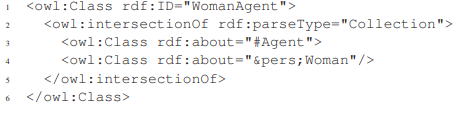
\includegraphics[width=.9\textwidth]{Figuras/op_and.PNG}
\caption{Operador intersectionOf}
\label{fig:opand}
\end{figure}


• \textit{owl:unionOf}: semelhante ao operador lógico OR, declara uma classe anônima cuja extensão de classe contém indivíduos que ocorrem em pelo menos uma extensão de classe das classes descritas em uma lista \cite{bechhofer2004}. Um exemplo de um trecho de código que utiliza este operador pode ser encontrado na Figura \ref{fig:opor}.

\begin{figure}[H]
\centering
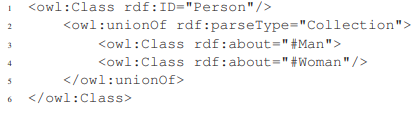
\includegraphics[width=.9\textwidth]{Figuras/op_or.PNG}
\caption{Operador unionOf}
\label{fig:opor}
\end{figure}


• \textit{owl:complementOf}: semelhante ao operador lógico NOT,  declara uma classe cuja extensão de classe contém exatamente os indivíduos que não pertencem à extensão de classe de outra classe, que é o objeto da declaração \cite{bechhofer2004}. Um exemplo de um trecho de código que utiliza este operador pode ser encontrado na Figura \ref{fig:opnot}.

\begin{figure}[H]
\centering
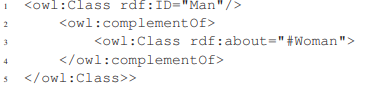
\includegraphics[width=.9\textwidth]{Figuras/op_not.PNG}
\caption{Operador complementOf}
\label{fig:opnot}
\end{figure}


\subsection{Sintaxe Manchester OWL}

A sintaxe \textit{Manchester OWL} \cite{horridge2006} foi criada para suprir a necessidade que algumas sintaxes geravam devido a falta de símbolos não-lógicos, pois, a maioria utiliza símbolos de lógica de descrição. Assim, a \textit{Manchester Sintax} fornecer aos casos em que são necessários utilizar símbolos não lógicos, uma sintaxe que facilita a criação de ontologias. Ela foi projetada principalmente para apresentar e editar expressões de classe em ferramentas, mas também pode ser usada para representar ontologias completas \cite{horridge2006}.

A Manchester OWL é uma sintaxe que de fácil utilização para para descrições OWL \cite{horridge2009}. Ela é influenciada tanto pela sintaxe \textit{Abstract OWL} quanto pela sintaxe \textit{DL style}, que usa símbolos lógicos de descrição, como o quantificador universal ($\forall$) ou o quantificador existencial ($\exists$). A sintaxe  Manchester usa símbolos matemáticos especiais como $\exists$, $\forall$, ¬ para serem substituídos por palavras-chave como “\textit{some}”, “\textit{only}” e “\textit{not}” respectivamente \cite{yauri2012}. Outro ponto diz respeito a palavra-chave \textit{"that"}, que possui a mesma função da palavra-chave \textit{"and"}, porém foi introduzida na sintaxe apenas para fazer com que a leitura das expressões fossem mais fluidas \cite{horridge2006}. Isso pode ser visto na Figura \ref{fig:manchester_exemplo}; onde existe \textit{"that"} pode ser substituído por \textit{"and"}, e vice-versa, e continuará com a mesma semântica.

Desde que o Manchester OWL Syntax foi criado, tornou-se a sintaxe padrão do \textit{Protégé} OWL \cite{horridge2006}. No caso do \textit{Protégé} \cite{noy2001}, ele estende a sintaxe para permitir uma apresentação ainda mais compacta em algumas situações (por exemplo, para explicação) \cite{horridge2009}.

Na Figura \ref{fig:manchester_exemplo} é possível ver a definição de uma expressão de classe. Essa expressão descreve um conjunto de pessoas que têm pelo menos um filho, que têm filhos que são apenas homens.

\begin{figure}[H]
\centering
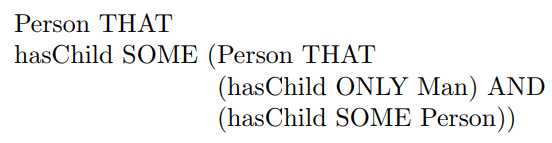
\includegraphics[width=0.5\textwidth]{Figuras/manchester_exemplo.png}
\caption{Exemplo de uma expressão de classe. Fonte: \cite{horridge2006}}
\label{fig:manchester_exemplo}
\end{figure}

\section{Processamento de Linguagem Natural}

O Processamento de Linguagem Natural é uma área de pesquisa e aplicação que explora como os computadores podem ser usados para entender e manipular texto ou discurso em linguagem natural para fazer coisas úteis. Os pesquisadores desta área buscam reunir conhecimentos sobre como os seres humanos entendem e usam a linguagem para que ferramentas e técnicas apropriadas possam ser desenvolvidas para fazer com que os sistemas de computador entendam e manipulem a linguagem natural para realizar as tarefas desejadas \cite{chowdhury2003}.

Em seu trabalho \cite{liddy2001} define PLN como uma gama teoricamente motivada de técnicas computacionais para analisar e representar textos que ocorrem naturalmente em um ou mais níveis de análise linguística com a finalidade de obter processamento de linguagem semelhante ao humano para uma série de tarefas ou aplicações.

\section{Lógica de Descrição}

Lógicas de descrição (DLs) são formalismos de representação de conhecimento baseados em lógica que são adaptados para representar o conhecimento terminológico de um domínio de aplicação de uma forma estruturada e formalmente bem compreendida. Eles permitem que seus usuários definam as noções (classes, relações, objetos) do domínio usando conceitos, funções e indivíduos; estabelecer restrições sobre o modo como essas noções podem ser interpretadas; e deduzir consequências, como subclasse e relacionamentos entre instâncias, das definições e restrições \cite{baader2001}.

As DLs tem sido empregadas em vários domínios de aplicações como processamento de linguagem natural, bancos de dados, ontologias. Porém, seu sucesso mais notável é provavelmente a adoção da linguagem OWL baseada em DL como linguagem de ontologia padrão para a web semântica \cite{baader2002}.

Uma DL pode ser caracterizada pelos construtores que ele fornece, por exemplo, a lógica ALC (\textit{Attributive Concept Language with Componentes} - Linguagem de Conceitos Atributivos com Componentes) é a DL que pode ter os construtores: união ($\sqcup$), intersecção ($\sqcap$), negação ($\neg$), restrição de valor ($\forall$), quantificação existencial ($\exists$) \cite{kepler2006}.

\section{Pellet}

A máquina de inferência Pellet, é implementado em Java e é \textit{open source}, ele fornece uma gama de recursos como: suporte a regras, conexão de raciocínio, identificação de axiomas. Para tornar seus recursos de raciocínio acessível aos usuários, ele fornece diferentes interfaces \cite{sirin2007}. 

Os recursos do Pellet são expostos a partir de uma API Java, uma interface de linha de comando ou um formulário da Web. Ele fornece acesso programático às funções de raciocínio por meio de duas interfaces diferentes, uma para o kit de ferramentas do Jena e uma para a biblioteca da API do OWL \cite{parsia2004}. No desenvolvimento da ferramenta em questão, o Pellet foi utilizado a partir de uma API Java e suas funções foram acessadas através da biblioteca do OWL. 

\begin{figure}[H]
\centering
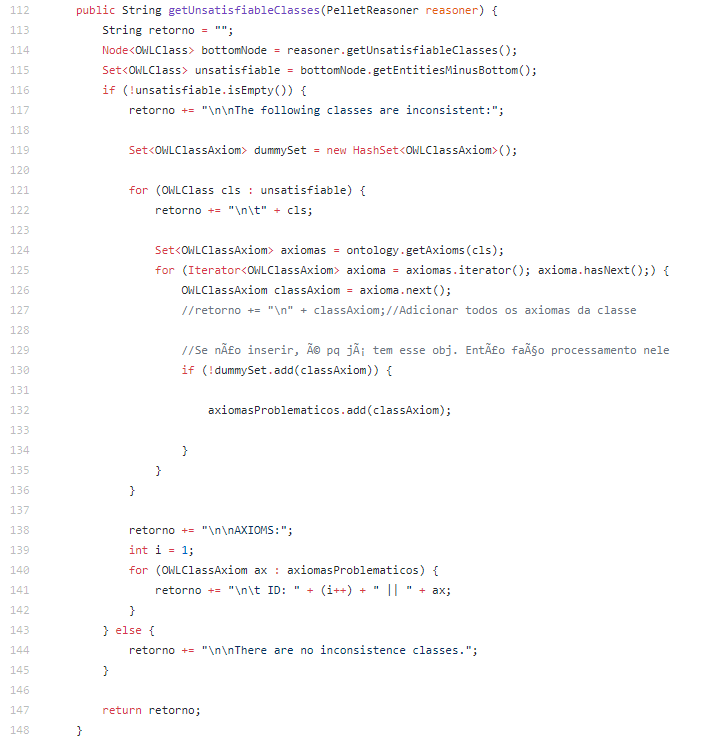
\includegraphics[width=1\textwidth]{Figuras/pellet_inconsistencia.png}
\caption{Código de procura por classes inconsistentes}
\label{fig:pellet_inconsistencia}
\end{figure}

Como é possível ver na Figura \ref{fig:pellet_inconsistencia}, a API fornece métodos que possibilitam fazer busca por inconsistência nos dados, a partir de um dado \textit{reasoner}, que por sua vez é criado a partir de uma ontologia. Ainda com a API do Pellet é possível inferir informação sobre uma ontologia, como é possível ver na Figura \ref{fig:pellet_inferencia}.


\begin{figure}[H]
\centering
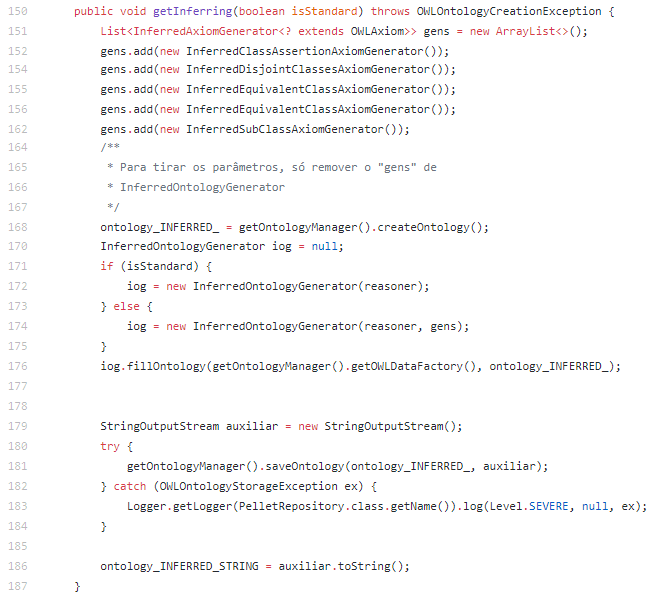
\includegraphics[width=1\textwidth]{Figuras/pellet_inferencia.png}
\caption{Exemplo de código inferindo informação sobre a ontologia}
\label{fig:pellet_inferencia}
\end{figure}

\section{Arquitetura Monolítica}

A arquitetura monolítica pode ser equiparada a uma aplicação composta por diversos módulos que são compilados de maneira separada e depois interligados, resultando num único e grande programa executável, onde cada módulo pode interagir de maneira livre. No modelo de arquitetura de camadas, o sistema é dividido em níveis sobrepostos. Cada uma dessas camadas possui um grupo de funções, elas só podem ser utilizadas por camadas que sejam superiores. Essa maneira de estruturação baseada em camadas cria uma hierarquia de níveis de acesso, o que pode ser uma vantagem pois fornece uma proteção paras as camadas mais internas, uma outra vantagem é a de isolar as funções, o que facilita na manutenção. Porém, esse modelo encontra uma desvantagem na questão do desempenho, pois, cada nova camada resulta numa mudança no modo de acesso \cite{machado2004}.


\section{Maven}

O Maven é uma ferramenta de integração de projetos Java utilizada no gerenciamento e automação de construção (build) de projetos, além disso, fornece diversas funcionalidades adicionais através do uso de \textit{plugins} e estimula o emprego de melhores práticas de programação \cite{maven}.

A ferramenta surgiu da dificuldades que muitos grupos de desenvolvimento tinham ao gerenciar bibliotecas em grandes projetos, de maneira dinâmica o Maven baixa a biblioteca Java e os seus \textit{plugins} de diversos repositórios que ficam armazenados em cache local, que pode ser atualizado quando sempre que for preciso \cite{oliveira2016}. Sua configuração é feita através do arquivo pom.xml (Project Object Model) onde são declarados o tipo de empacotamento, suas dependências e os repositórios de onde as dependências serão buscadas, podendo ser tanto repositórios locais ou remotos. \cite{junior2014}

A Figura \ref{fig:pom_xml} mostra um trecho do arquivo pom.xml utilizado na implementação da OrCA. É possível ver definições de compilação, como por exemplo a versão do Java que será utilizado, a classe principal que será executada ao projeto ser iniciado, o tipo de empacotamento, versão e id (pacote) que serão utilizados na publicação desses arquivos para o repositório local do maven, bem como as dependências utilizadas pelo projeto.

\begin{figure}[H]
\centering
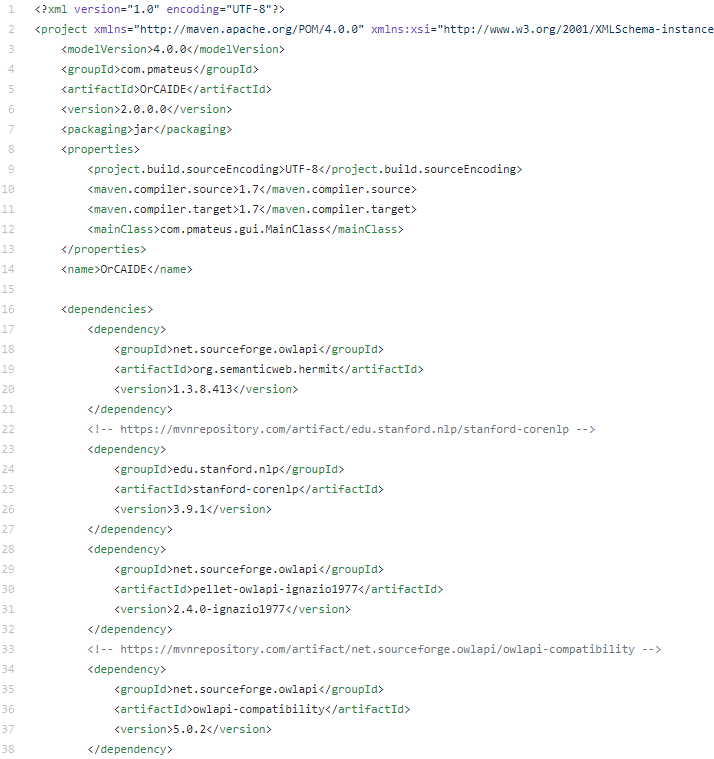
\includegraphics[width=1\textwidth]{Figuras/pom_xml.png}
\caption{Trecho de arquivo pom.xml da \textit{OrCA}}
\label{fig:pom_xml}
\end{figure}

\section{Compilador}

De maneira geral, um compilador é um programa que tem como entrada um código de programa numa certa linguagem e produz como saída um código de programa numa outra linguagem, preservando o significado do código durante esse processo \cite{grune2012}.

Um compilador é dividido em fases, cada uma delas representam uma etapa do processo de compilação, elas podem ser desenvolvidas de maneira separada, mesmo que na prática elas funcionem intercaladamente \cite{foleiss2009}. 

Em seu livro, \cite{somerville2003} faz uma definição geral, onde ele afirma que os compiladores de linguagem de programação possuem uma arquitetura genérica, ela pode ser dividida em componentes como os ilustrados na Figura \ref{fig:compiladorl}.

\begin{figure}[H]
\centering
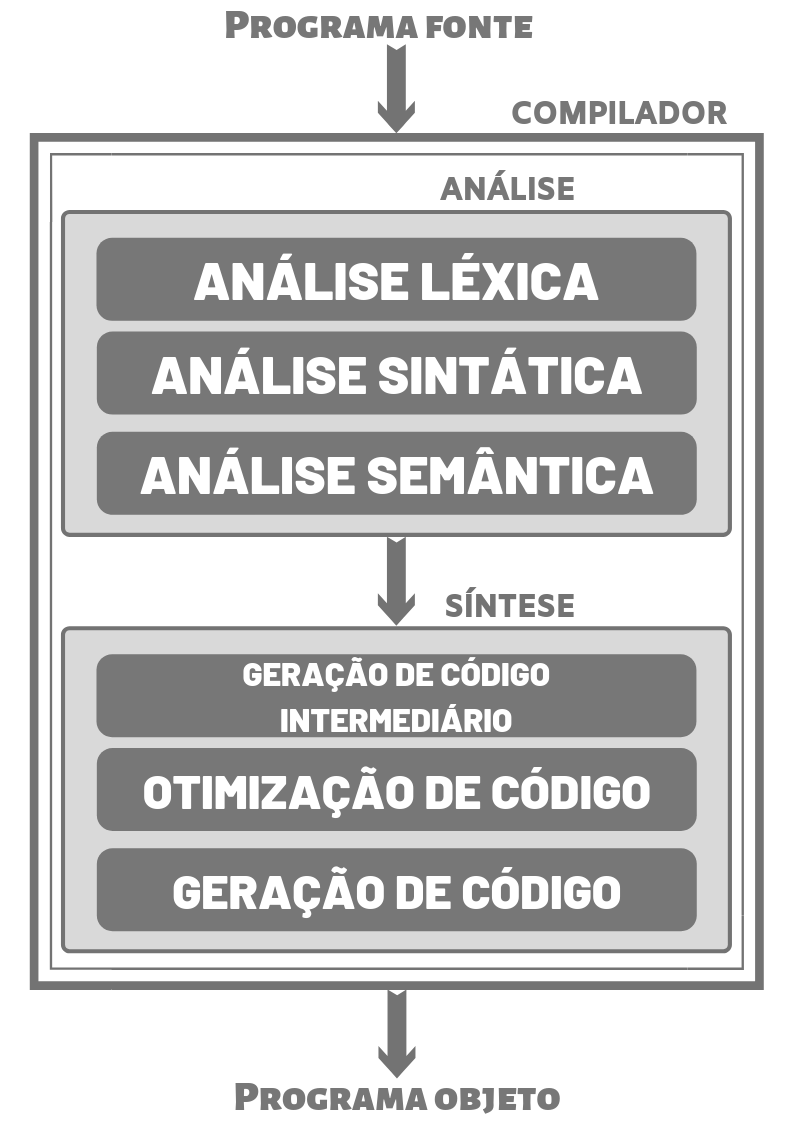
\includegraphics[width=.6\textwidth]{Figuras/compilador.png}
\caption{Fases do compilador}
\label{fig:compiladorl}
\end{figure}

• \textbf{Analisador Léxico}: recebe como entrada o código fonte e sua função é ler os caracteres deste código e categorizar suas sequências em \textit{tokens}, que são unidades lógicas denominadas que em seguida serão utilizadas por outras partes do compilador, como o
analisador sintático \cite{foleiss2009}. Um \textit{token} é uma sequência de caracteres que pode ser tratada como uma unidade na gramática de uma linguagem de programação, que por sua vez classifica os \textit{tokens} em um conjunto finito de tipos de \textit{token} \cite{andrew2002}.

Na fase de análise léxica, o analisador utiliza um fluxo de caracteres e produz um fluxo de nomes, palavras-chave e sinais de pontuação, ele descarta espaço em branco e comentários entre os \textit{tokens}, a presença de espaços em branco e comentários, complicaria indevidamente o analisador \cite{andrew2002}.

Diversas atividades com grande importância são realizadas durante essa análise, as que mais se destacam são: conversão numérica, identificação de palavras reservadas, e criação e manutenção das tabelas de símbolos, que serão muito utilizadas durante o processo de compilação \cite{neto2017};

• \textbf{Tabela de Símbolos}: possui informações sobre os nomes das entidades (variáveis, nomes de classes, nomes de objetos etc.) usadas no texto que está sendo traduzido \cite{somerville2003};

• \textbf{Analisador Sintático}: responsável pela análise sintática, o analisador sintático recebe como entrada uma cadeia de \textit{tokens} que foi gerada pelo analisador léxico, e faz a verificação para confirmar se ela pode ser gerada pela gramática da linguem em questão. Assim, espera-se que o analisador mostre qualquer erro de sintaxe \cite{aho2007}. Para isso, ele faz uso da gramática da linguagem que foi pré definida e então constrói uma árvore de sintaxe \cite{somerville2003};

• \textbf{Árvore Sintática}: é uma estrutura interna utilizada para representar o programa a ser compilado \cite{somerville2003};

• \textbf{Analisador Semântico}: realiza a verificação da correção semântica das instruções, a análise é feita através de regras que são previamente definidas e então disparadas durante a fase análise sintática. De modo similar, regras de geração de código são associadas à estrutura sintática da linguagem. O código gerado implementa as operações especificadas pelo programa na linguagem de saída do compilador \cite{barbosa2009}.

A fase de análise semântica de um compilador conecta definições de variáveis a seus usos, verifica se cada expressão tem um tipo correto e traduz a sintaxe abstrata em uma representação mais simples adequada para gerar código de máquina \cite{andrew2002};

• \textbf{Gerador de Código}: percorre a árvore sintática e sem seguida gera códigos de máquina abstrata \cite{somerville2003};

Cada linguagem de programação possui uma gramática, que consiste em símbolos terminais, símbolos não-terminais, um símbolo inicial e produções. Símbolos terminais são os símbolos básicos a partir dos
quais as cadeias são formadas \cite{ferreira2015}.

\chapter{Arquitetura do Sistema}
\label{chap:sistema}

\section{Introdução}
Com a finalidade de criar ontologias a partir de Processamento de Linguagem Natural (PLN), o sistema OrCA (\textit{Ontology vieweR and CreAtor}) foi desenvolvido. Neste capítulo descrevemos detalhes da arquitetura do sistema e suas funcionalidades, bem com a linguagem natural controlada (LNC) utilizada para criação das ontologias. O intuito, ao definir esta LNC, foi facilitar ao máximo o desenvolvimento das ontologias por parte dos usuários do sistema. Na Figura \ref{fig:diagComponenteGeral} é possível observar o diagrama de componentes do sistema. O componente \textit{Ontology} depende do componente \textit{Compiler}, o componente \textit{Reasoner} depende do componente \textit{Compiler}. Já o componente \textit{Graph Viewer} depende do componente \textit{Ontology}. O componente \textit{Compiler} é o principal componente do sistema, no qual todos os demais componentes possuem dependência direta ou indireta.

\begin{figure}[H]
\centering
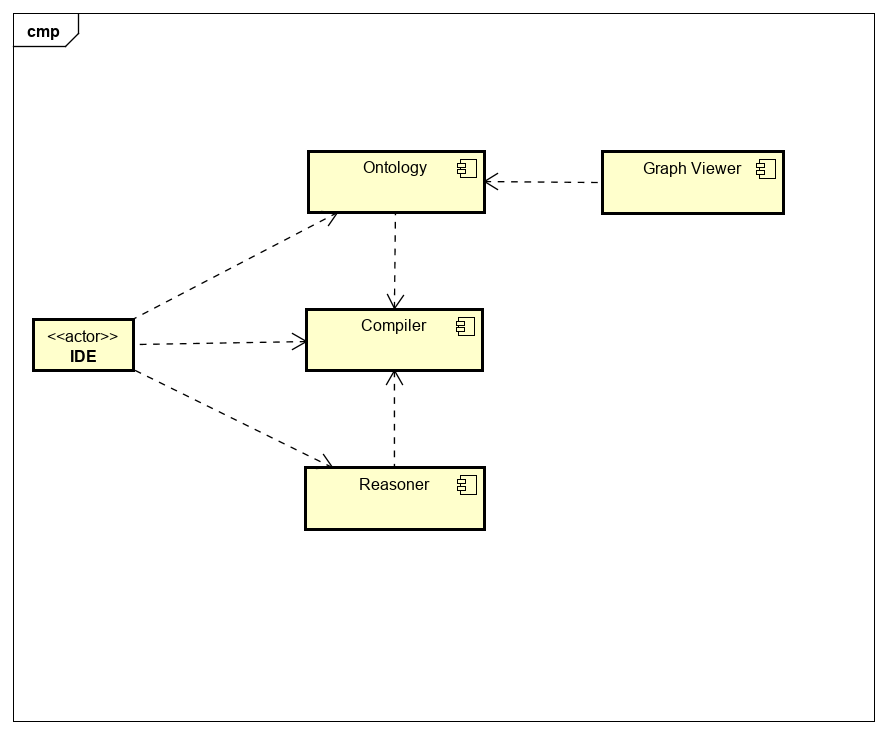
\includegraphics[width=.63\textwidth]{Figuras/DiagramadeComponentes.png}
\caption{Diagrama de componentes geral}
\label{fig:diagComponenteGeral}
\end{figure}

\section{Arquitetura}

O sistema foi implementado utilizando a arquitetura monolítica, visando otimizar o desenvolvimento e facilitar a manutenção do código fonte. Qualquer desenvolvedor e/ou programador que visualizar a estrutura do projeto e desejar realizar ajustes, não terá dificuldades em achar seus componentes. Na Figura \ref{fig:pacotesJava} é possível visualizar todos os pacotes do projeto.

\begin{figure}[H]
\centering
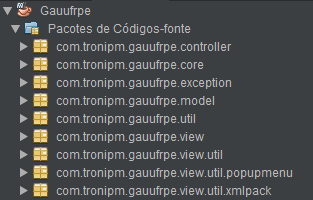
\includegraphics[width=.6\textwidth]{Figuras/estrutura.png}
\caption{Pacotes de classes no projeto}
\label{fig:pacotesJava}
\end{figure}

\section{Componentes}
O sistema possui 4 componentes (telas): \textit{Compiler}, \textit{Ontology}, \textit{Reasoner} e \textit{Graph Viewer}. Detalhes de cada componente do sistema serão vistos nas subseções seguintes. Todos os componentes que serão descritos a seguir podem ser localizados no pacote exibido na Figura \ref{fig:pacotesView}. 

\begin{figure}[H]
\centering
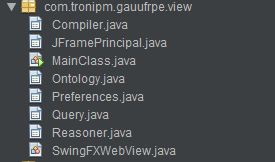
\includegraphics[width=.6\textwidth]{Figuras/pacote_view.png}
\caption{Pacote contendo os principais componentes.}
\label{fig:pacotesView}
\end{figure}

\subsection{Componente Compiler}

O \textit{compiler} é responsável por receber a LNC do usuário e retornar se essa LNC pode ou não ser compilada, bem como apresentar eventuais erros que impossibilitam a compilação. A Tela completa pode ser vista na Figura \ref{fig:telaCompiler}.


\begin{figure}[H]
\centering
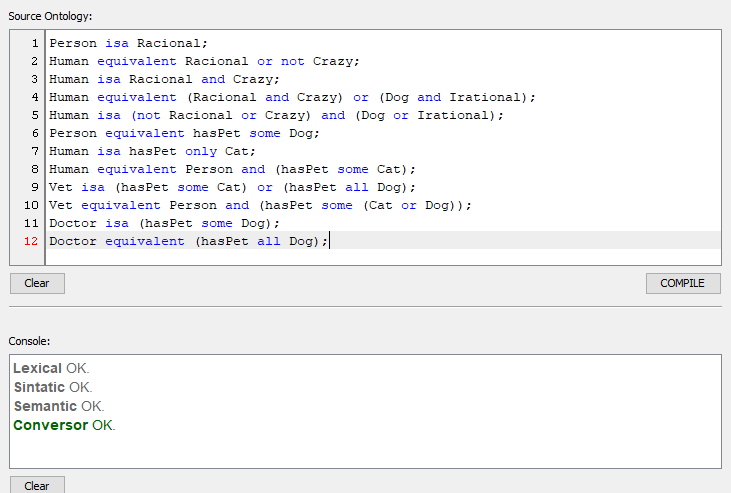
\includegraphics[width=.8\textwidth]{Figuras/tela_compiler.png}
\caption{Tela \textit{Compiler} completa}
\label{fig:telaCompiler}
\end{figure}

Como apresentado na Figura \ref{fig:telaCompiler1}, o campo de texto chamado \textit{Source Ontology} é onde o usuário irá inserir as sentenças usando a LNC desenvolvida. O botão \textit{Clear} tem a função de apagar todo o conteúdo desse campo de texto, e o botão \textit{COMPILE} faz a compilação das sentenças em ontologias.

\begin{figure}[H]
\centering
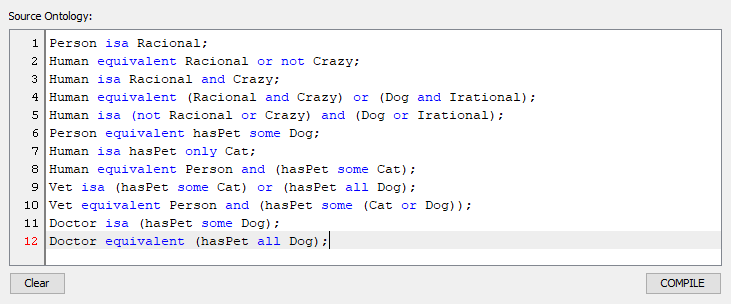
\includegraphics[width=.8\textwidth]{Figuras/tela_compiler1.png}
\caption{Tela \textit{Compiler}: parte da edição da Linguagem Natural}
\label{fig:telaCompiler1}
\end{figure}

Na mesma tela, porém no campo Console (Vide Figura \ref{fig:telaCompiler2}), é possível ver a saída do compilador com uma mensagem amigável para o usuário. Há 5 tipos de saídas no console: 

\begin{enumerate}
  \item \textbf{Lexical OK}: passou sem erros pelo analisador léxico;
  \item \textbf{Sintatic OK}: passou sem erros pelo analisador sintático;
  \item \textbf{Semantic OK}: passou sem erros pelo analisador semântico;
  \item \textbf{Conversor OK}: a linguagem utilizada pelo usuário foi convertida com sucesso para uma ontologia.
  \item \textbf{Erros}: ao passo que algum erro seja encontrado, o console (Figura \ref{fig:telaCompiler2}) irá mostrar em qual linha, coluna e palavra aconteceu o erro.
\end{enumerate}

\begin{figure}[H]
\centering
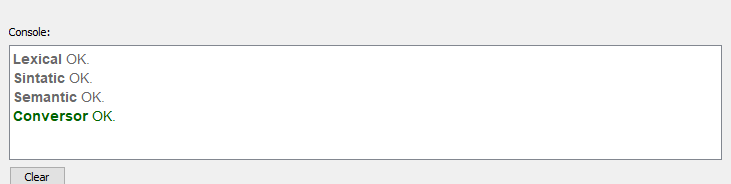
\includegraphics[width=.8\textwidth]{Figuras/tela_compiler2.png}
\caption{Tela \textit{Compiler}: retorno da compilação da linguagem natural}
\label{fig:telaCompiler2}
\end{figure}

\subsection{Componente Ontology}
\label{sec:compOntology}

A \textit{Ontology} mostra a saída da ontologia (em OWL) após a compilação das sentenças dadas pelos usuários. Este campo não é editável, porém, embora o usuário não possa inserir ou remover texto, o modelo de visualização pode ser alterado através do menu suspenso chamado \textit{Output Model} para as seguintes sintaxes: \textit{RDF/XML} (padrão), \textit{KRSS2, Latex, Manchester OWL Syntax, OWL/XML, OWL Functional Syntax} e \textit{Turtle}. Todas essas sintaxes são fornecidas pela \textit{Manchester OWL API}. 

O botão \textit{Graph} tem a função de abrir o componente \textit{Graph}, e o botão \textit{Copy} a de enviar o texto que está aparecendo no campo de texto para a área de transferência. Na Figura \ref{fig:telaOntology} é possível observar a Tela \textit{Ontology} completa.

\begin{figure}[H]
\centering
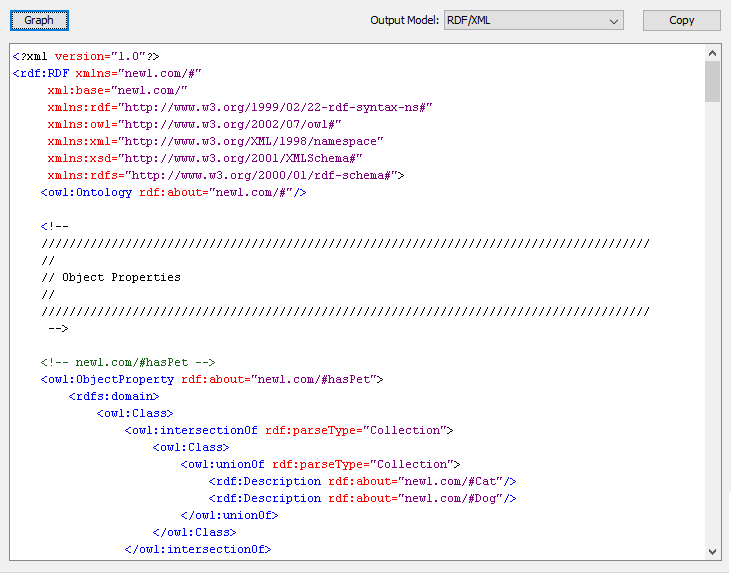
\includegraphics[width=.8\textwidth]{Figuras/tela_ontology.png}
\caption{Tela Ontology}
\label{fig:telaOntology}
\end{figure}

\subsection{Componente Reasoner}

Se tratando de ontologias, uma máquina de inferência (\textit{reasoner}) é um \textit{software} capaz de inferir consequências lógicas sobre uma ontologia. O campo de texto superior do componente \textit{Reasoner} apresenta a saída (Deduções e Inconsistências) que o \textit{reasoner} integrado a máquina de inferência (\textit{Pellet}) consegue realizar.

O botão \textit{Reason} refaz o processamento de deduzir sobre a ontologia base. O campo de texto \textit{Ontology Inferred} é o código \textit{OWL} da nova ontologia criada a partir dos axiomas deduzidos. O botão \textit{Save on Text File} tem a função de abrir uma caixa de diálogo permitindo que o usuário salve essa nova ontologia em seu computador. Apresentamos na Figura \ref{fig:telaReasoner} a tela completa. Os casos de uso da tela \textit{Ontology} são apresentados na Figura \ref{fig:ucontology}. 

\begin{figure}[H]
\centering
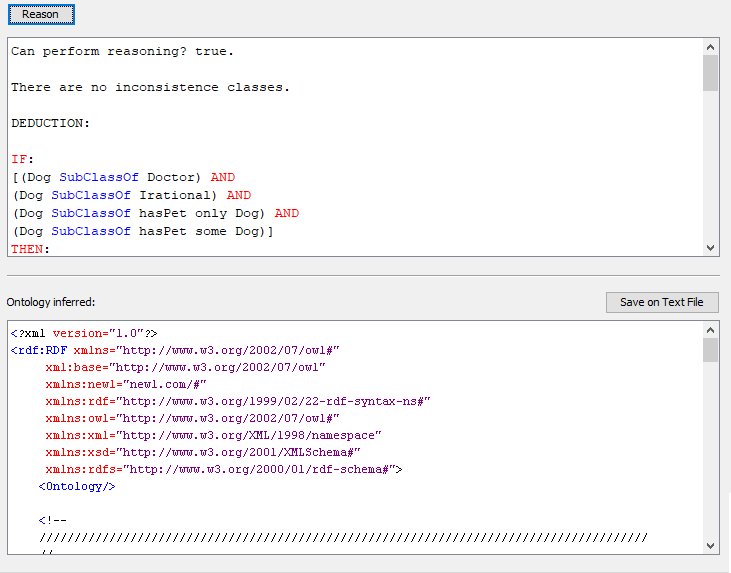
\includegraphics[width=.8\textwidth]{Figuras/tela_reasoner.png}
\caption{Tela Reasoner}
\label{fig:telaReasoner}
\end{figure}

\begin{figure}[H]
\centering
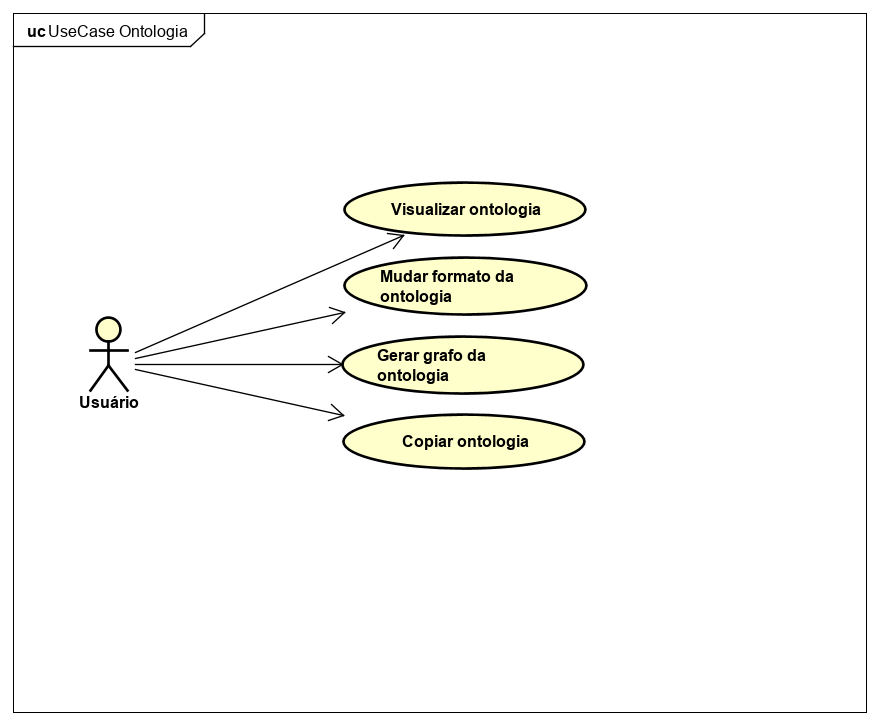
\includegraphics[width=.6\textwidth]{Figuras/UseCaseOntologia.png}
\caption{Caso de Uso da tela \textit{Ontology}} 
\label{fig:ucontology}
\end{figure}

\subsection{Componente Graph Viewer}

O componente \textit{Graph Viewer} é apenas um facilitador gráfico, a fim de mostrar a ontologia compilada em forma de grafo. Apresentamos na Figura \ref{fig:telGraph} a tela \textit{Graph Viewer}, que é responsável por apresentar ao usuário uma perspectiva de grafo da ontologia criada a partir das sentenças em LNC. Nela é possível aumentar e diminuir zoom, assim como exportar tanto em arquivo de imagem no formato SVG como em texto no formato JSON. É possível também movimentar os nós, bem como aumentar ou diminuir o tamanho desses, para facilitar a visualização. 

\begin{figure}[H]
\centering
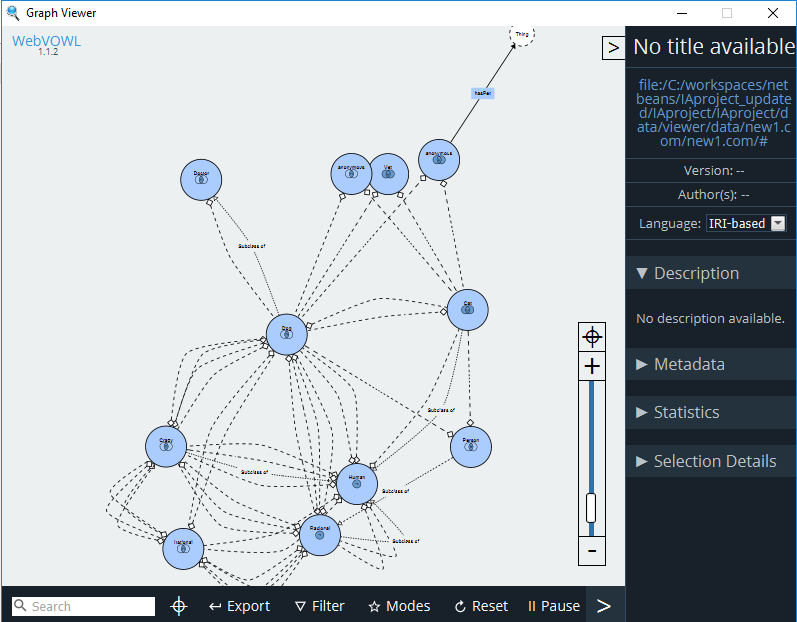
\includegraphics[width=.7\textwidth]{Figuras/tela_graph.png}
\caption{Tela Graph Viewer}
\label{fig:telGraph}
\end{figure}

Os casos de uso da tela \textit{Graph Viewer} são apresentados na Figura \ref{fig:ucgv}.

\begin{figure}[H]
\centering
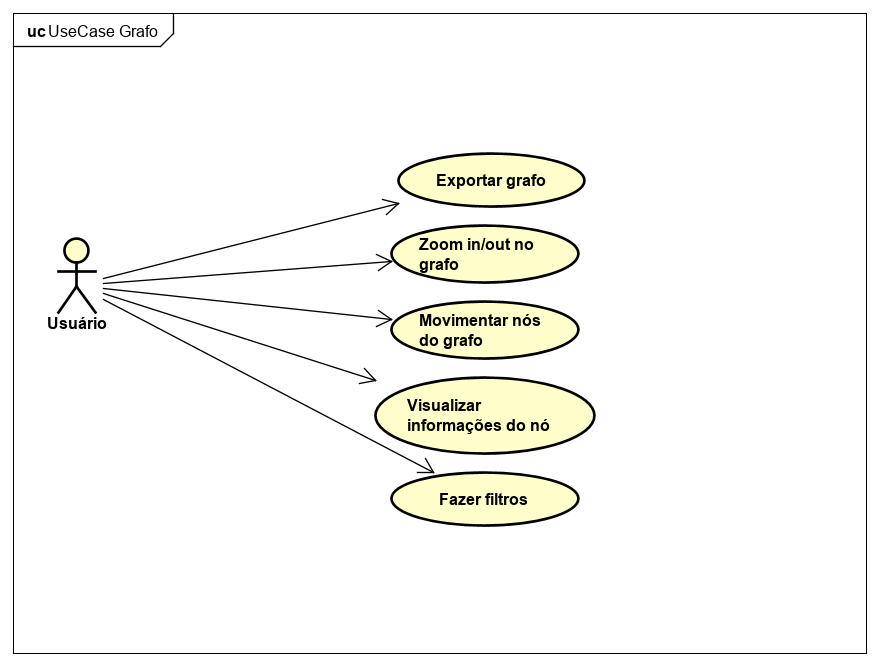
\includegraphics[width=.7\textwidth]{Figuras/UseCaseGrafo.png}
\caption{Caso de Uso da tela \textit{Graph Viewer}} 
\label{fig:ucgv}
\end{figure}

\section{Componente Compilador}

Um compilador é um tipo de programa que traduz um código descrito em alto nível, ou seja, mais legível e fácil de entender pelo ser humano, em um código semanticamente equivalente em baixo nível, não legível pelo ser humano e não necessariamente executável pela máquina. Geralmente um compilador não traduz imediatamente um código de máquina, mas sim um código intermediário, em linguagem simbólica, só a partir deste momento o código é traduzido para uma linguagem de máquina \cite{grune2012}. De forma semelhante, o compilador desenvolvido para a OrCA não irá traduzir o código descrito pelo usuário para um código de máquina, mas sim para um código "intermediário", o \textit{OWL 2 DL}, que para os fins desse projeto já é o código final.

Para um programa ser definido como um compilador, ele precisa ter alguns processos, são eles: análise léxica, análise sintática, análise semântica e conversor. Juntos, esses quatro processos formam  o ciclo necessário para um compilador verificar se o código descrito pelo usuário não possui erros e pode ser compilado. O fluxo de um compilador padrão pode ser observado na Figura \ref{fig:compilerscheme}.

\begin{figure}[H]
\centering
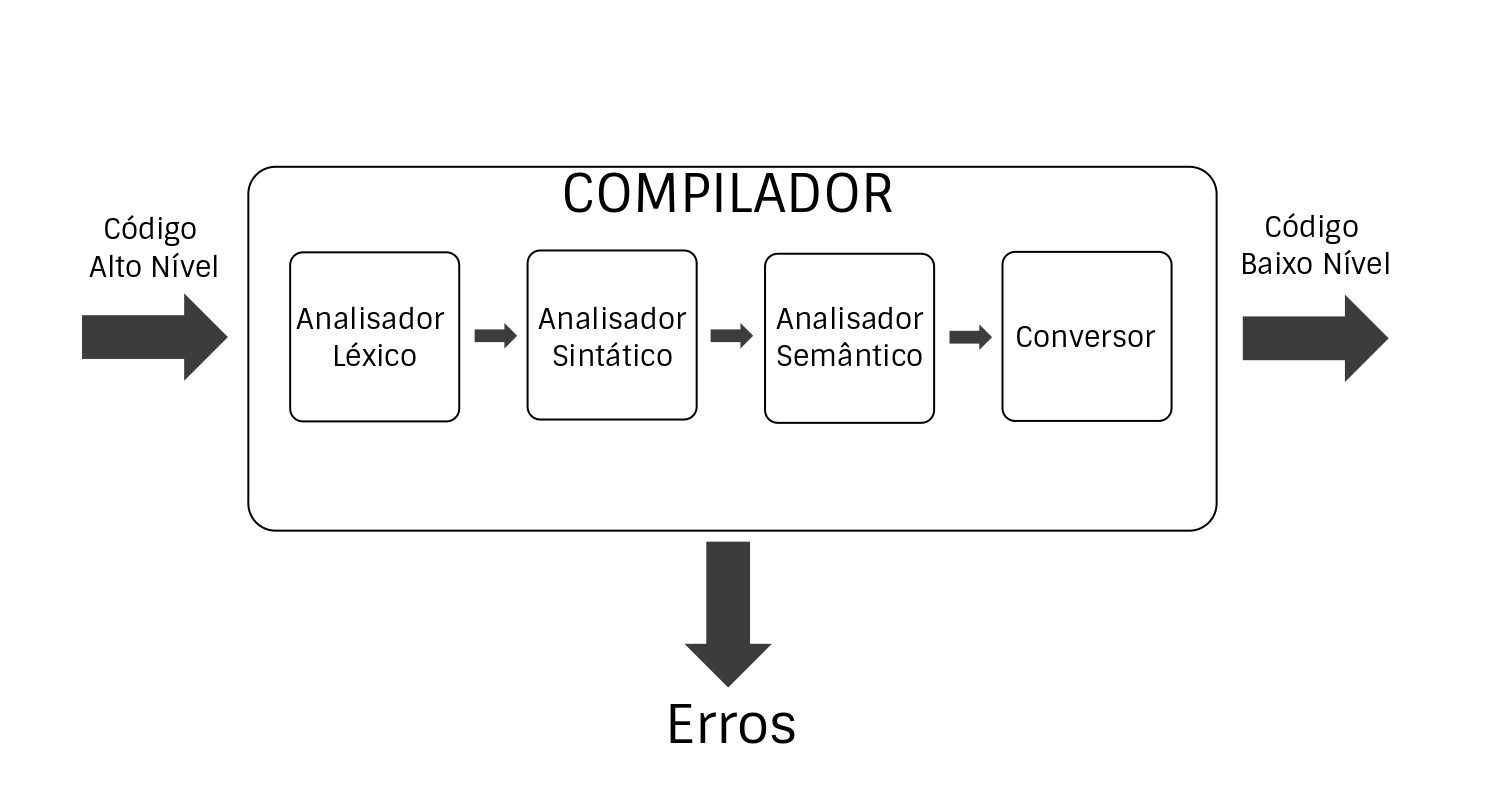
\includegraphics[width=.8\textwidth]{Figuras/compiladorscheme.png}
\caption{Fluxo de um compilador}
\label{fig:compilerscheme}
\end{figure}

O fluxo que o compilador OrCA segue é o mesmo de um compilador padrão. Inicialmente o código é examinado pelo Analisador Léxico, caso haja algum erro que esse analisador possa detectar, o processo de compilação é suspenso, e é informado ao usuário, na tela \textit{Compiler} > \textit{Console}, a linha e a posição onde o erro ocorreu. Caso as verificações desse analisador não detectem erro o próximo passo é iniciado, o Analisador Sintático. Neste passo, acontece de igual forma ao Analisador Léxico, porém, ele faz suas próprias verificações. Caso não sejam detectados erros, o passo seguinte é inicializado, o Analisador Semântico. De maneira semelhante aos passos anteriores, o Analisador Semântico faz suas próprias verificações e análises. Se nenhum erro for encontrado, a próxima etapa é iniciada, a conversão. Nesta fase, as sentenças em LNC inseridas pelos usuários, passam por todo o processo apresentado de compilação e o resultado é um código \textit{OWL 2 DL}. Na Figura \ref{fig:uclnc} é possível verificar os casos de uso dessa tela.

\begin{figure}[H]
\centering
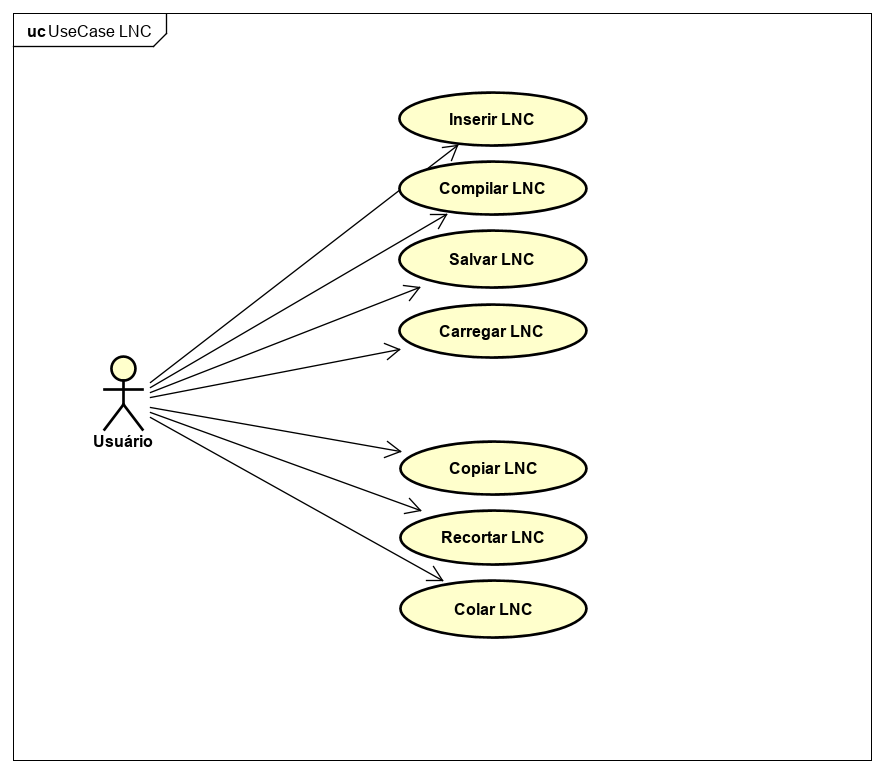
\includegraphics[width=.6\textwidth]{Figuras/UseCaseLNC.png}
\caption{Caso de Uso da tela \textit{Compiler}} 
\label{fig:uclnc}
\end{figure}


\subsection{Gramática}

Idiomas como o português, inglês e espanhol possuem um conjunto de regras e normas bem definidas. Isto permite que pessoas com conhecimento destas regras comuniquem-se entre si, tanto no ato de escrever como no de ler. O conjunto dessas regras é chamado gramática. Assim como em um idioma normal, um compilador precisa de regras e normas gramaticais. Isso garante que, ao usuário escrever seu código, ele será entendido por outras pessoas, assim como pelo compilador. Na Tabela \ref{tab:tabelaGramatica} é possível observar a gramática definida para o compilador OrCA. Cada linha é chamada de Regra de Produção. A coluna da esquerda é o título da regra, enquanto a coluna da direita é a regra em si. Para fins de leitura, chamada de regra é feita com <...>, por exemplo <OP>. Chamada de terminal é feita sem <...>, por exemplo \textit{some} ou (. O Símbolo "||" é apenas um separador entre as regras.

\begin{table}[H]
\centering
\begin{tabular}{l|l}
Regra  & Definição  \\ 
\hline <OP>  & \begin{tabular}[l]{@{}l@{}} some || all || only || and || or || isa || equivalent || that || disjoint \end{tabular} \\
\hline <ID>  & \begin{tabular}[l]{@{}l@{}} a-Z* \end{tabular} \\
\hline <NUM> & \begin{tabular}[l]{@{}l@{}} 0-9* \end{tabular} \\
\hline <FIM> & \begin{tabular}[l]{@{}l@{}} ; || <DEF> || $\varepsilon$ \end{tabular} \\ 
\hline <DEF> & 
\begin{tabular}[l]{@{}l@{}} 
<ID> <OP> <ID> <FIM> \textbf{||} \\
<ID> <OP> (<DEF>) <FIM> || \\
(<DEF>) <OP> <ID> <FIM> || \\
<ID> <OP> <DEF> <FIM> || \\
\end{tabular} \\
\end{tabular} 
\caption{Gramática OrCA IDE}
\label{tab:tabelaGramatica}
\end{table} 


\section{Linguagem Natural Controlada}
\label{sec:lnc}

Para que o usuário consiga utilizar o sistema, se faz necessário que ele possua o conhecimento da LNC que será definida a seguir, na Tabela \ref{tab:tabelaPalavrasReservadas} observamos as palavras reservadas, suas respectivas descrições e um exemplo de sua aplicação.

\begin{table}[H]
\centering
\begin{tabular}{l|l|l}
 Reservado  & Descrição & Exemplo  \\ 
\hline isa & \begin{tabular}[l]{@{}l@{}} Uma classe X é um \\tipo de classe Y.\end{tabular} & Gato isa Felino \\ \hline
equivalent & \begin{tabular}[l]{@{}l@{}} Uma classe X é um tipo \\ de classe irmã de Y.\end{tabular} & JanelaBanheiro equivalent JanelaCasa \\ \hline and / that & \begin{tabular}[l]{@{}l@{}} Uma classe X interseção\\ com uma classe Y.\end{tabular} & (Correr and Pular) isa ExercicioFisico  \\ \hline or & \begin{tabular}[l]{@{}l@{}}Uma classe X disjunção\\ de uma classe Y. \end{tabular} & Trabalhar isa nor(Dormir or Comer) \\ \hline only & \begin{tabular}[l]{@{}l@{}}Uma propriedade X\\ only classe Y. \end{tabular} & podeLatir only Cachorro \\ \hline some & \begin{tabular}[l]{@{}l@{}}Uma propriedade X\\ some classe Y. \end{tabular} & andarNoMuro some Gato \\ \hline all & \begin{tabular}[l]{@{}l@{}}Uma propriedade X \\ all classe Y. \end{tabular} & comerGrama all Vaca \\ \hline not & Negação de uma Classe & not Gato \\ \hline nor & Negação de uma expressão & nor(Gato isa Felino) \\ \hline disjoint & Uma classe X é disjunção da classe Y & Ferrari disjoint BMW \\
\end{tabular}
\caption{Palavras Reservadas}
\label{tab:tabelaPalavrasReservadas}
\end{table}

Como visto de maneira resumida na Tabela \ref{tab:tabelaPalavrasReservadas}, na Figura \ref{fig:codigoFonteInicial} está o código fonte que o sistema mostra ao ser aberto, para que o usuário entenda o funcionamento da sintaxe.

\begin{figure}[H]
\centering
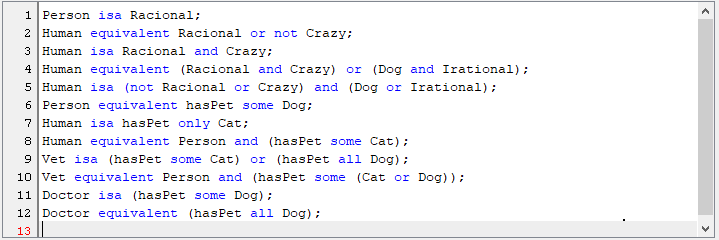
\includegraphics[width=.8\textwidth]{Figuras/codigo_codigofonte_inicial.png}
\caption{Código inicial}
\label{fig:codigoFonteInicial}
\end{figure}

\subsection{Analisador Léxico}

Este analisador é responsável por fazer o primeiro e menos complexo processamento sobre o código, em LNC, inserido pelo usuário. Esse processamento nada mais é do que receber o texto da interface gráfica e verificar se as palavras e símbolos inseridos pelo usuário são válidos, ou seja, se são aceitos pela gramática do compilador. Essas palavras e símbolos podem ser vistos na Figura \ref{fig:codigoTokenenum}. Com exceção de \textit{END}, \textit{NUMBER} e \textit{IDENTIFIER}, cada palavra e símbolo desta imagem é chamado de "palavra reservada", e não podem ser utilizados para outro fim se não o que foi definido pela gramática deste compilador. O tipo \textit{NUMBER} diz respeito a uma numeração, que pode variar de 1 a ±\textit{n}, ou seja, um número qualquer, já o \textit{IDENTIFIER} diz respeito a uma palavra, que não é reservada pelo compilador, mas foi criada pelo usuário, por exemplo "Cachorro" ou "Vaca". \textit{END} significa que é o final do código inserido pelo usuário. Cada palavra e/ou símbolo inserido pelo usuário é chamado de \textit{token}.

\begin{figure}[H]
\centering
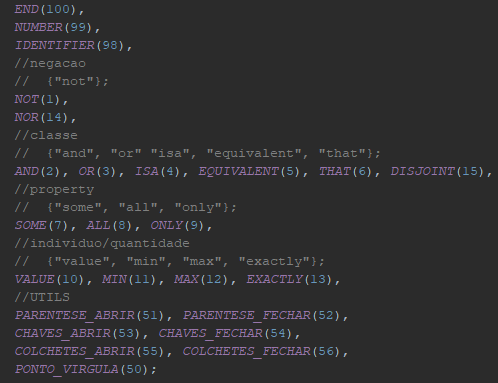
\includegraphics[width=.6\textwidth]{Figuras/codigo_tokenenum.png}
\caption{Palavras reservadas e símbolos permitidos pela gramática}
\label{fig:codigoTokenenum}
\end{figure}

A análise léxica consiste em verificar todos os \textit{tokens}. Caso o \textit{token} não pertença a nenhum dos tipos apresentados na Figura \ref{fig:codigoTokenenum}, irá apresentar uma exceção do tipo \textit{LexicalAnalyzerException}, e o processo de compilação será forçadamente parado (ver Figura \ref{fig:codigoErroLexico}). Caso este \textit{token} pertença a algum dos tipos, ele é adicionado em uma lista de \textit{tokens}. Ao final da análise, essa lista é passada para o Analisador Sintático, encerrando esta análise e mostrando ao usuário que esta etapa foi finalizada com sucesso (ver Figura \ref{fig:codigoSucessoLexico}).

\begin{figure}[H]
\centering
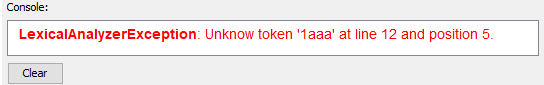
\includegraphics[width=.8\textwidth]{Figuras/codigo_erro_lexico.png}
\caption{Erro do Analisador Léxico sendo mostrado ao usuário na Tela \textit{Compiler}}
\label{fig:codigoErroLexico}
\end{figure}

\begin{figure}[H]
\centering
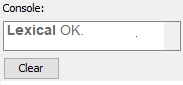
\includegraphics[width=.3\textwidth]{Figuras/codigo_sucesso_lexico.png}
\caption{Analisador Léxico foi executado com sucesso}
\label{fig:codigoSucessoLexico}
\end{figure}

\subsection{Analisador Sintático}

Após a análise léxica, o analisador sintático é acionado. Ele é responsável por identificar se o código inserido pelo usuário faz parte da gramática que o compilador aceita. Em outras palavras, enquanto o analisador léxico se preocupa em verificar se as palavras são aceitas pelo compilador, o analisador sintático verifica se as palavras foram utilizadas na posição correta. Em alguns casos é utilizado \textit{look ahead} de 1 ou 2 tokens para garantir que a leitura na pilha de execução seja a esperada pelo sistema. A Figura \ref{fig:codigoLookAhead} traz um trecho de código do analisador sintático mostrando a utilização de \textit{look ahead}. Esse código verifica se o item atual da pilha é um \textit{not} e, utilizando 1 \textit{token} de \textit{look ahead}, verifica se o próximo item é um \textit{identifier}, e, utilizando mais 1 \textit{token} de \textit{look ahead}, verifica se esse próximo \textit{token} é um operador (\textit{OR}, \textit{AND}, \textit{ISA}, etc).
 
\begin{figure}[H]
\centering
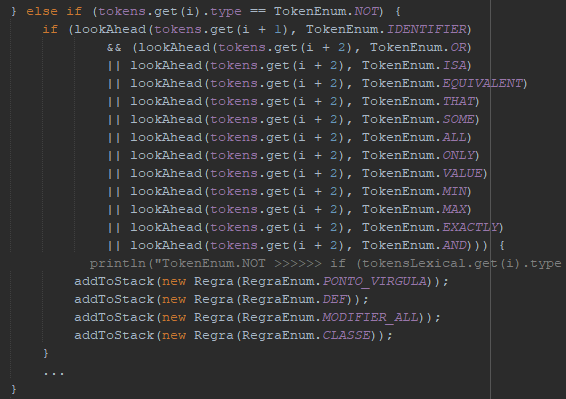
\includegraphics[width=.8\textwidth]{Figuras/codigo_lookahead.png}
\caption{Trecho de código mostrando a utilização do \textit{look ahead}. }
\label{fig:codigoLookAhead}
\end{figure}

Caso alguma expressão do código inserido pelo usuário não pertença a gramática aceita pelo compilador, uma exceção do tipo \textit{SintaticAnalyzerException} será lançada, como é possível observar na Figura \ref{fig:codigoErroSintatico}. Caso o código do usuário respeite a gramática, esse passo será encerrado, mostrando ao usuário uma mensagem de sucesso como a exibida na Figura \ref{fig:codigoSucessoSintatico}.

\begin{figure}[H]
\centering
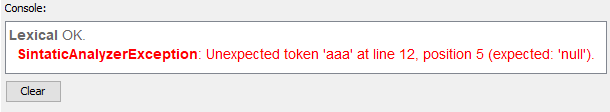
\includegraphics[width=.8\textwidth]{Figuras/codigo_erro_sintatico.png}
\caption{Erro do Analisador Sintático sendo mostrado ao usuário na Tela \textit{Compiler}}
\label{fig:codigoErroSintatico}
\end{figure}

\begin{figure}[H]
\centering
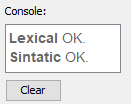
\includegraphics[width=.3\textwidth]{Figuras/codigo_sucesso_sintatico.png}
\caption{Analisador Sintático foi executado com sucesso}
\label{fig:codigoSucessoSintatico}
\end{figure}

\subsection{Analisador Semântico}

Posterior a análise sintática esse componente entra em ação. Ele tem um comportamento diferente dos analisadores semânticos de outros compiladores. A função dele é atomizar o código fonte inserido pelo usuário a fim de criar sub expressões de tamanho mínimo, por exemplo "Homem and Mulher", embora essa expressão faça parte de uma expressão maior denominada "(Homem and Mulher) isa Humano". Essa substituição pode ser vista na Figura \ref{fig:codigoAtomizacao} onde se encontra o código do arquivo ControllerSemantic.java que exibe o momento em que a atomização envolvendo essas palavras reservadas é feita. 

\begin{figure}[H]
\centering
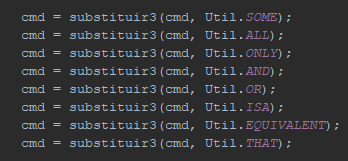
\includegraphics[width=.7\textwidth]{Figuras/codigo_atomizacao.png}.
\caption{Código atomização}
\label{fig:codigoAtomizacao}
\end{figure}

Cada expressão atomizada é inserida em uma lista que será enviada para o ControllerConversor. Caso aconteça algum erro na atomização, uma exceção do tipo SemanticAnalyzerException será lançada na view, como é possível observar na Figura \ref{fig:codigoErroSemantico}. Caso o código fonte seja atomizado com sucesso, irá passar para o Controller Conversor.

\begin{figure}[H]
\centering
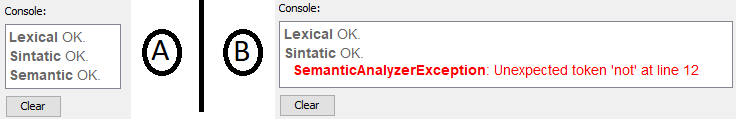
\includegraphics[width=.7\textwidth]{Figuras/codigo_erro_semantico.png}
\caption{Erro Semântico}
\label{fig:codigoErroSemantico}
\end{figure}

A Figura \ref{fig:codigoErroSemantico} está dividida em duas partes, a parte A mostra quando o código passa com sucesso pelo analisador semântico e a parte B mostra quando houve um erro ao tentar atomizar o código fonte.


\subsection{Conversor}

Esse componente é responsável por converter a linguagem natural inserida pelo usuário em uma ontologia 2 DL. Ao chegar nesse ponto, todas as verificações referentes a análise léxica, sintática e semântica já foram feitas, garantindo que não ocorrerá nenhum tipo de erro no que diz respeito a linguagem natural inserida.

A Figura \ref{fig:codigoConversor} exibe o trecho de código em que ocorre o processo inicial de conversão das expressões AND e THAT, é nessa parte onde é feita a separação quando a expressão é CLASSE vs CLASSE, ou CLASSE vs EXPRESSÃO (vice-versa) ou ainda, EXPRESSÃO vs EXPRESSÃO.

\begin{figure}[H]
\centering
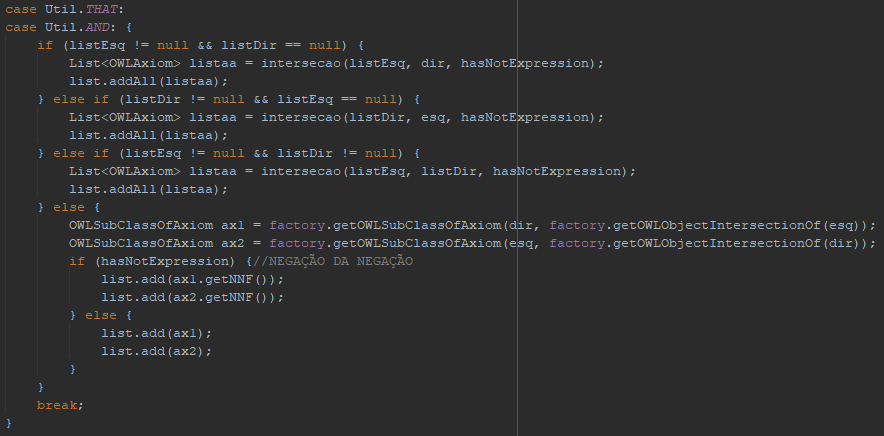
\includegraphics[width=.8\textwidth]{Figuras/codigo_conversor_andthat.png}
\caption{Trecho de código} 
\label{fig:codigoConversor}
\end{figure}

\subsection{Funcionalidades}
O sistema possui algumas funcionalidades básicas no menu contextual (clique direito do mouse sobre o painel) ou na barra de ferramentas (Menu > \textit{Edit}), podendo variar de acordo com o painel, são elas: Copiar, Colar, Cortar, Selecionar tudo, Limpar, Desfazer e Refazer (ver Figura \ref{fig:uclnc}). Na tela \textit{Compiler} o usuário pode inserir sua Linguagem Natural Controlada, bem como compilar, salvar, carregar,  além das opções do menu contextual. 

A tela \textit{Ontology} fornece ao usuário, além das opções do menu contextual: visualizar a ontologia proveniente da sua LNC e mudar formato da ontologia (RDF/XML, Latex, etc), ver Figura \ref{fig:ucontology}.

Na tela \textit{Graph Viewer} é possível aumentar/diminuir zoom, movimentar nós, visualizar informações do nó, exportar o grafo (Json e PNG) e fazer filtros para simplificar o grafo, entre outros. Ver Figura \ref{fig:ucgv}.


\subsection{Considerações Finais}
Concluímos que a ferramenta foi criada com o intuito de facilitar a criação de ontologias por pessoas sem conhecimento em linguagens de programação. Os componentes analisadores - léxico, sintático e semântico - garantem que a linguagem natural inserida seja equivalente a ontologia resultante após a compilação. Podemos perceber também que, pelo fato do usuário poder selecionar o tipo de sintaxe da ontologia, isso possibilita utilizar essa informação para leitura humana (mais fácil de compreender) ou para utilização em outros \textit{softwares} (com informações mais complexas).


\chapter{Experimentos e Resultados}
\label{chap:exp}

Os experimentos realizados tiveram como principal objetivo verificar a capacidade da ferramenta desenvolvida em cumprir com os objetivos propostos, essa verificação se deu através da análise dos resultados que foram coletados durante a execução dos experimentos. Aqui são apresentados o planejamento das etapas que foram realizadas, o material e métodos que foram utilizados, planejamento da amostra e os resultados obtidos.


\section{Delineamento Experimental}
O experimento realizado foi dividido em três etapas: 

\textbf{Etapa um}: nesta etapa foi verificada a capacidade da ferramenta de construir ontologias a partir da linguagem natural controlada (Vide Capítulo 3, Seção 3.5). Para que tivéssemos um resultado seguro e confiável, foi selecionado uma ontologia já existente com conceitos claros e bem definidos. Desta forma, ao tentar reproduzir esta ontologia, já é possível saber qual deverá ser o resultado final. O próximo passo foi criar o código na sintaxe da OrCA para descrever esta ontologia. Como grande parte dos axiomas desta ontologia são de baixa complexidade, um filtro com apenas os axiomas mais complexos foi criado, selecionando axiomas com base no quantitativo de classes envolvidas em sua definição. Após este código criado ser executado no OrCA, o resultado foi comparado com a ontologia original, a fim de saber se foi possível recriá-la com a mesma expressividade, ou seja, com os mesmos axiomas.

\textbf{Etapa dois}: consistiu nos testes do módulo de raciocínio, verificando a capacidade da OrCA de realizar raciocínio e checar inconsistências. Como foram utilizados axiomas de uma ontologia real, não existiam inconsistências, desta forma, foram criados axiomas específicos para gerar inconsistências e testar a capacidade da OrCA em realizar esse tipo de raciocínio. Diferente da etapa um, a ontologia inteira\footnote{Com as restrições que serão impostas na Seção \ref{sec:materialemetodo}} foi utilizada nesta etapa. Todos os axiomas foram executados na OrCA e no \textit{Protégé}. O código OWL obtido nas duas ferramentas foi comparado, desta forma foi possível ter um resultado confiável entre uma ferramenta amplamente utilizada por profissionais e a ferramenta desenvolvida.

\textbf{Etapa três}: esta etapa foi baseada em testar o módulo de inferência da ferramenta, constatando se ela é capaz de inferir novos axiomas a ontologia, ou seja, se a ferramenta é capaz deduzir algum conhecimento novo da ontologia que não está explícito. Os axiomas utilizados neste passo foram os mesmos da etapa anterior, porém sem os axiomas inconsistentes. Para ter um resultado confiável, o resultado da OrCA para esta etapa também foi comparado ao resultado do \textit{Protégé}, este também utilizando os mesmos axiomas.

\section{Material e Métodos}
\label{sec:materialemetodo}
% COLOCAR TIL NO  MEIO DA LINHA {\raise.17ex\hbox{$\scriptstyle\sim$}}

Uma vez definidas as etapas a serem realizadas na fase de experimentos, se faz necessária a escolha do material a ser utilizado. Para que tenhamos um resultado final controlado e confiável, foi escolhido uma ontologia já existente, com axiomas bem definidos e validada por profissionais, assim, mesmo no início do experimento é possível saber qual deverá ser o resultado obtido pela a OrCA, visto que para uma ontologia ser igual a outra, ela precisa conter os mesmos axiomas. Logo, o código OWL gerado pela OrCA precisa ser o mesmo da ontologia original. 

A ontologia selecionada foi a  NTDO\footnote{\url{http://www.cin.ufpe.br/\~ntdo/}} (\textit{Neglected Tropical Disease Ontology} - Ontologia de Doenças Tropicais Negligenciadas) \cite{ntdo}. Ela tem o objetivo representar um domínio com relevância e impacto reconhecido pela literatura e por instituições de saúde pública. Nela, é modelada em detalhes o processo de transmissão de doenças e o falecimento de indivíduos a partir dessas doenças \cite{ntdo}.

Todos os axiomas que foram utilizados nos experimentos e que formam nossa base de dados experimental, foram extraídos da ontologia NTDO. Uma vez que a OrCA é focado em axiomas de expressividade ALC, foram considerados unicamente axiomas relacionados a subclasses, equivalência de classes, definição de classe, disjunção de classes e definição de propriedades (Vide Tabelas \ref{tab:QtdALSNTDO} e \ref{tab:QtdConstNTDO}). É importante ressaltar também que a OrCA não trata axiomas com cardinalidade e utiliza os construtores de união ($\sqcup$), interseção ($\sqcap$), negação (¬), restrição universal ($\forall$) e restrição existencial ($\exists$) (Vide Tabela \ref{tab:QtdConstNTDO}).

\begin{table}[H]
\centering
\begin{tabular}{l|l}
Tipo Axioma       & Quantidade \\ \hline
SubClassOf        & 48         \\ \hline
EquivalentClasses & 5          \\ \hline
DisjointClasses   & 1          \\
\end{tabular}
\caption{Quantitativo de axiomas extraídos da NTDO}
\label{tab:QtdALSNTDO}
\end{table}

\begin{table}[H]
\centering
\begin{tabular}{l|l}
Construtor & Quantidade \\ \hline
And        & 9          \\ \hline
Or         & 4          \\ \hline
Some       & 6          \\ \hline
All\footnotemark        & 11         \\ \hline
Not        & 1         \\
\end{tabular}
\caption{Quantitativo de construtores extraídos da NTDO}
\label{tab:QtdConstNTDO}
\end{table}

\footnotetext{é o equivalente ao construtor \textit{Only} no \textit{Protégé}, quantificador universal}

\begin{table}[H]
\centering
\begin{tabular}{l|l}
Tipo Objeto   & Quantidade \\ \hline
Class         & 57         \\ \hline
Property      & 12         \\
\end{tabular}
\caption{Quantitativo de classes e propriedades extraídos da NTDO.}
\label{tab:QtdObjsNTDO}
\end{table}

O código OWL completo da ontologia extraída pode ser visto no Apêndice \ref{chap:apOntologia}.3. Nas Tabelas \ref{tab:QtdALSNTDO}, \ref{tab:QtdConstNTDO} e \ref{tab:QtdObjsNTDO} é possível ver o quantitativo da amostra extraída. Originalmente, a ontologia NTDO é composta por seis arquivos: \textit{ntdo.owl}\footnote{\url{http://www.cin.ufpe.br/~ntdo/OWLFiles/ntdo.owl}}, \textit{InjuryAndDeath.owl}\footnote{\url{http://www.cin.ufpe.br/~ntdo/OWLFiles/InjuryAndDeath.owl}}, \textit{Leishmaniasis.owl}\footnote{\url{http://www.cin.ufpe.br/~ntdo/OWLFiles/Leishmaniasis.owl}}, \textit{DengueFever.owl}\footnote{\url{http://www.cin.ufpe.br/~ntdo/OWLFiles/DengueFever.owl}}, \textit{CID-10.owl}\footnote{\url{http://www.cin.ufpe.br/~ntdo/OWLFiles/CID-10.owl}} e \textit{GeoOnto.owl}\footnote{\url{http://www.cin.ufpe.br/~ntdo/OWLFiles/GeoOnto.owl}}, porém apenas o arquivo \textit{ntdo.owl} foi utilizado, uma vez que este arquivo possui objetos suficientes para o experimento.

\begin{figure}[H]
\centering
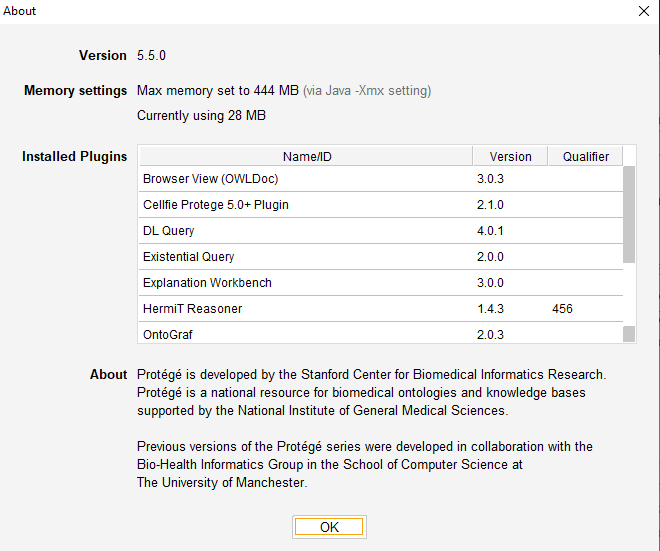
\includegraphics[width=.5\textwidth]{Figuras/protege.png}
\caption{Versão e plugins pre-instalados no \textit{Protégé} } 
\label{fig:protege}
\end{figure}

O \textit{Protégé} utilizado nos experimentos está na versão 5.5.0, como pode ser visto na Figura \ref{fig:protege}. Nenhum componente ou plugin foi adicionado, além dos que são instalados juntamente com a ferramenta (plugins \textit{default}).

\section{Planejamento da Amostra}

Uma vez que a maioria dos axiomas desta ontologia é de complexidade baixa, algo como  $X \subseteq Y$ (X é subclasse de Y), apenas axiomas com 3 ou mais classes envolvidas serão utilizados para demonstração. Após este filtro, 8 axiomas foram selecionados. O quantitativo de axiomas, construtores e objetos, após o filtro, podem ser observados respectivamente nas Tabelas \ref{tab:QtdALSNTDO_filtro}, \ref{tab:QtdConstNTDO_filtro} e \ref{tab:QtdObjsNTDO_filtro}. 
\begin{table}[H]
\centering
\begin{tabular}{l|l}
Tipo Axioma       & Quantidade \\ \hline
SubClassOf        & 13         \\ \hline
EquivalentClasses & 1          \\ \hline
DisjointClasses   & 1          \\ 
\end{tabular}
\caption{Quantitativo de axiomas extraídos da NTDO após filtro}
\label{tab:QtdALSNTDO_filtro}
\end{table}

\begin{table}[H]
\centering
\begin{tabular}{l|l}
Construtor & Quantidade \\ \hline
And        & 6          \\ \hline
Or         & 4          \\ \hline
Some       & 6          \\ \hline
All        & 11         \\ \hline
Not        & 1         \\ 
\end{tabular}
\caption{Quantitativo de construtores da NTDO após filtro}
\label{tab:QtdConstNTDO_filtro}
\end{table}

\begin{table}[H]
\centering
\begin{tabular}{l|l}
Tipo Objeto   & Quantidade \\ \hline
Class         & 19         \\ \hline
Property      & 12         \\ 
\end{tabular}
\caption{Quantitativo de classes e propriedades da NTDO após filtro}
\label{tab:QtdObjsNTDO_filtro}
\end{table}

O código OWL completo da ontologia resultante após essa restrição pode ser visto no Apêndice \ref{chap:apOntologia}.4. As subseções seguintes mostrarão todos os axiomas selecionados em OWL, assim como em representação DL, e na sintaxe OrCA. 

\section{Etapa um}

Nesta sessão serão mostrados todos os axiomas resultantes ao filtro criado. Cada axioma será exibido em OWL, forma original em que foi extraído, e será chamado de código OWL. Também na sintaxe OrCA, uma vez que para que um axioma seja processado pela ferramenta, ele precisa estar na sintaxe descrita no Capítulo \ref{chap:sistema}, Seção \ref{sec:lnc}, e será chamado de código OrCA, e por fim na representação DL. Os códigos OrCA são as entradas do sistema. Os códigos OWL mostrados fazem parte da ontologia original, e serão usados como comparativo, logo, a saída da OrCA deverá conter o mesmo código OWL. Como mostrado no Capítulo \ref{chap:sistema}, Seção \ref{sec:compOntology}, código OWL também é o formato da saída da ferramenta.

\subsection{Axioma 1}
O axioma pode ser visto na representação DL na figura \ref{fig:axioma1_dl}. O código OrCA deste axioma, que será usado como entrada, pode ser visto na figura \ref{fig:axioma1_orca}. E a Figura \ref{fig:axioma1_o} mostra a forma original deste axioma (em OWL) que será usado para comparação. 

\begin{figure}[H]
\centering
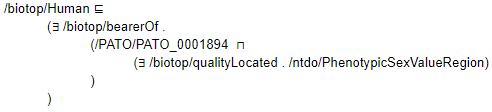
\includegraphics[width=.7\textwidth]{Figuras/axioma1_dl.png}
\caption{Axioma 1 na representação DL} 
\label{fig:axioma1_dl}
\end{figure}

\begin{figure}[H]
\centering
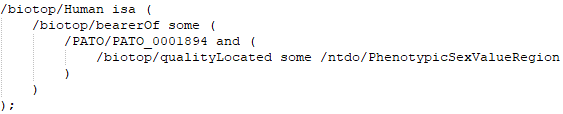
\includegraphics[width=.7\textwidth]{Figuras/axioma1_orca.png}
\caption{Axioma 1 na sintaxe OrCA} 
\label{fig:axioma1_orca}
\end{figure}

\begin{figure}[H]
\centering
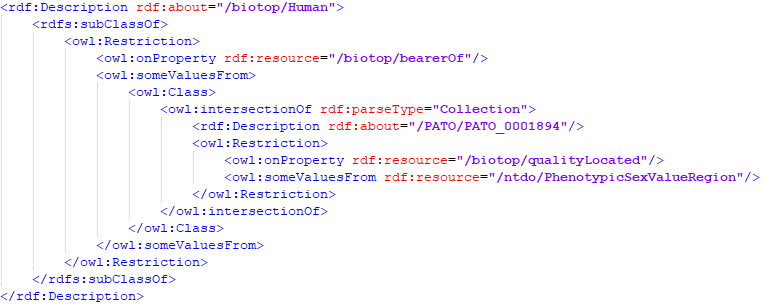
\includegraphics[width=.8\textwidth]{Figuras/axioma1_o.png}
\caption{Axioma 1 retirado da NTDO} 
\label{fig:axioma1_o}
\end{figure}

A OrCA teve a mesma saída do código OWL mostrado na Figura \ref{fig:axioma1_o}, assim sendo, não é necessário mostrar o mesmo código, visto que eles são idênticos, porém ele pode ser visto no Apêndice \ref{chap:apOntologia}.2.

\subsection{Axioma 2}
O axioma pode ser visto na representação DL na figura \ref{fig:axioma2_dl}. O código OrCA deste axioma, que será usado como entrada, pode ser visto na figura \ref{fig:axioma2_orca}. E a Figura \ref{fig:axioma2_o} mostra a forma original deste axioma (em OWL) que será usado para comparação. 

\begin{figure}[H]
\centering
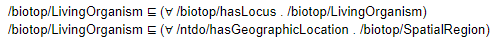
\includegraphics[width=.7\textwidth]{Figuras/axioma2_dl.png}
\caption{Axioma 2 na representação DL} 
\label{fig:axioma2_dl}
\end{figure}

\begin{figure}[H]
\centering
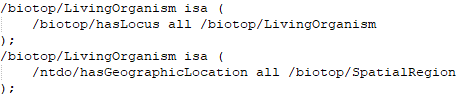
\includegraphics[width=.7\textwidth]{Figuras/axioma2_orca.png}
\caption{Axioma 2 na sintaxe OrCA} 
\label{fig:axioma2_orca}
\end{figure}

\begin{figure}[H]
\centering
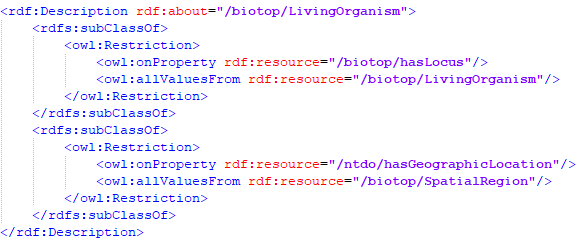
\includegraphics[width=.8\textwidth]{Figuras/axioma2_o.png}
\caption{Axioma 2 retirado da NTDO} 
\label{fig:axioma2_o}
\end{figure}

A OrCA teve a mesma saída do código OWL mostrado na Figura \ref{fig:axioma2_o}, assim sendo, não é necessário exibir o mesmo código, visto que eles são idênticos, porém ele pode ser visto no Apêndice \ref{chap:apOntologia}.2.

\subsection{Axioma 3}
O axioma pode ser visto na representação DL na figura \ref{fig:axioma3_dl}. O código OrCA deste axioma, que será usado como entrada, pode ser visto na figura \ref{fig:axioma3_orca}. E a Figura \ref{fig:axioma3_o} mostra a forma original deste axioma (em OWL) que será usado para comparação. 

\begin{figure}[H]
\centering
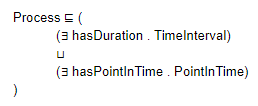
\includegraphics[width=.5\textwidth]{Figuras/axioma3_dl.png}
\caption{Axioma 3 na representação DL} 
\label{fig:axioma3_dl}
\end{figure}

\begin{figure}[H]
\centering
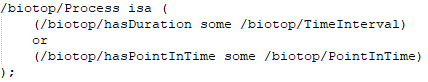
\includegraphics[width=.7\textwidth]{Figuras/axioma3_orca.png}
\caption{Axioma 3 na sintaxe OrCA} 
\label{fig:axioma3_orca}
\end{figure}

\begin{figure}[H]
\centering
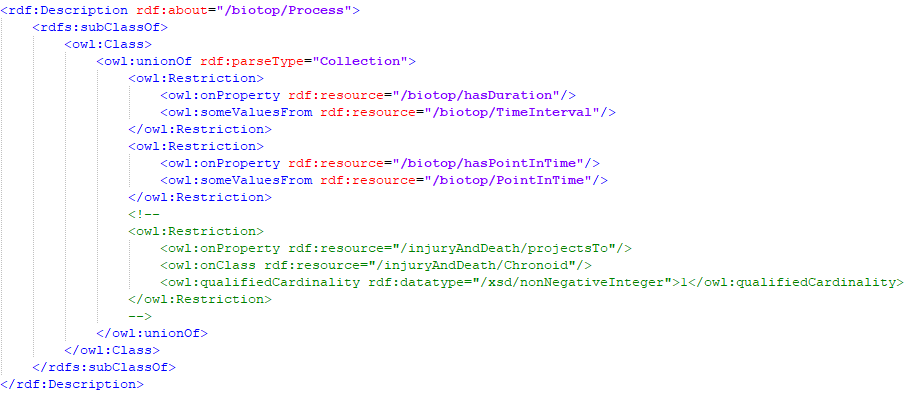
\includegraphics[width=.9\textwidth]{Figuras/axioma3_o.png}
\caption{Axioma 3 retirado da NTDO} 
\label{fig:axioma3_o}
\end{figure}

Ao ignorar a cardinalidade, a OrCA teve a mesma saída do código OWL mostrado na Figura \ref{fig:axioma3_o}, assim sendo, não é necessário exibir o mesmo código, visto que eles são idênticos, porém ele pode ser visto no Apêndice \ref{chap:apOntologia}.2.

\subsection{Axioma 4}
O axioma pode ser visto na representação DL na figura \ref{fig:axioma4_dl}. O código OrCA deste axioma, que será usado como entrada, pode ser visto na figura \ref{fig:axioma4_orca}. E a Figura \ref{fig:axioma4_o} mostra a forma original deste axioma (em OWL) que será usado para comparação. 

\begin{figure}[H]
\centering
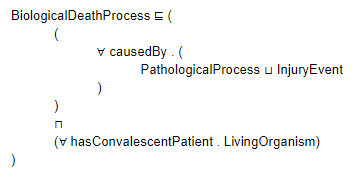
\includegraphics[width=.6\textwidth]{Figuras/axioma4_dl.png}
\caption{Axioma 4 na representação DL} 
\label{fig:axioma4_dl}
\end{figure}

\begin{figure}[H]
\centering
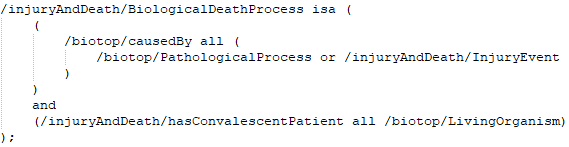
\includegraphics[width=.7\textwidth]{Figuras/axioma4_orca.png}
\caption{Axioma 4 na sintaxe OrCA} 
\label{fig:axioma4_orca}
\end{figure}

\begin{figure}[H]
\centering
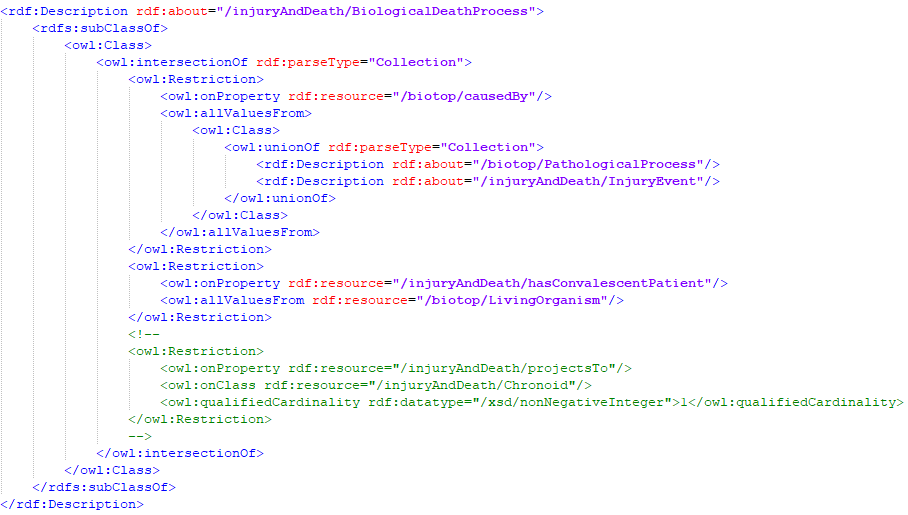
\includegraphics[width=1\textwidth]{Figuras/axioma4_o.png}
\caption{Axioma 4 retirado da NTDO} 
\label{fig:axioma4_o}
\end{figure}

Ao ignorar a cardinalidade, a OrCA teve a mesma saída do código OWL mostrado na Figura \ref{fig:axioma4_o}, assim sendo, não é necessário exibir o mesmo código, visto que eles são idênticos, porém ele pode ser visto no Apêndice \ref{chap:apOntologia}.2.

\subsection{Axioma 5}
O axioma pode ser visto na representação DL na figura \ref{fig:axioma5_dl}. O código OrCA deste axioma, que será usado como entrada, pode ser visto na figura \ref{fig:axioma5_orca}. E a Figura \ref{fig:axioma5_o} mostra a forma original deste axioma (em OWL) que será usado para comparação. 

\begin{figure}[H]
\centering
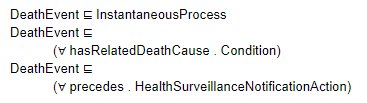
\includegraphics[width=.6\textwidth]{Figuras/axioma5_dl.png}
\caption{Axioma 5 na representação DL} 
\label{fig:axioma5_dl}
\end{figure}

\begin{figure}[H]
\centering
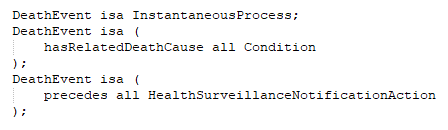
\includegraphics[width=.7\textwidth]{Figuras/axioma5_orca.png}
\caption{Axioma 5 na sintaxe OrCA} 
\label{fig:axioma5_orca}
\end{figure}

\begin{figure}[H]
\centering
\includegraphics[width=.8\textwidth]{Figuras/axioma5_o.png}
\caption{Axioma 5 retirado da NTDO} 
\label{fig:axioma5_o}
\end{figure}

A OrCA teve a mesma saída do código OWL mostrado na Figura \ref{fig:axioma5_o}, assim sendo, não é necessário exibir o mesmo código, visto que eles são idênticos, porém ele pode ser visto no Apêndice \ref{chap:apOntologia}.2.

\subsection{Axioma 6}
O axioma pode ser visto na representação DL na figura \ref{fig:axioma6_dl}. O código OrCA deste axioma, que será usado como entrada, pode ser visto na figura \ref{fig:axioma6_orca}. E a Figura \ref{fig:axioma6_o} mostra a forma original deste axioma (em OWL) que será usado para comparação. 

\begin{figure}[H]
\centering
\includegraphics[width=.7\textwidth]{Figuras/axioma6_dl.png}
\caption{Axioma 6 na representação DL} 
\label{fig:axioma6_dl}
\end{figure}

\begin{figure}[H]
\centering
\includegraphics[width=.7\textwidth]{Figuras/axioma6_orca.png}
\caption{Axioma 6 na sintaxe OrCA} 
\label{fig:axioma6_orca}
\end{figure}

\begin{figure}[H]
\centering
\includegraphics[width=1\textwidth]{Figuras/axioma6_o.png}
\caption{Axioma 6 retirado da NTDO} 
\label{fig:axioma6_o}
\end{figure}

A OrCA teve a mesma saída do código OWL mostrado na Figura \ref{fig:axioma6_o}, assim sendo, não é necessário exibir o mesmo código, visto que eles são idênticos, porém ele pode ser visto no Apêndice \ref{chap:apOntologia}.2.

\subsection{Axioma 7}
O axioma pode ser visto na representação DL na figura \ref{fig:axioma7_dl}. O código OrCA deste axioma, que será usado como entrada, pode ser visto na figura \ref{fig:axioma7_orca}. E a Figura \ref{fig:axioma7_o} mostra a forma original deste axioma (em OWL) que será usado para comparação. 

\begin{figure}[H]
\centering
\includegraphics[width=.6\textwidth]{Figuras/axioma7_dl.png}
\caption{Axioma 7 na representação DL} 
\label{fig:axioma7_dl}
\end{figure}

\begin{figure}[H]
\centering
\includegraphics[width=.7\textwidth]{Figuras/axioma7_orca.png}
\caption{Axioma 7 na sintaxe OrCA} 
\label{fig:axioma7_orca}
\end{figure}

\begin{figure}[H]
\centering
\includegraphics[width=1\textwidth]{Figuras/axioma7_o.png}
\caption{Axioma 7 retirado da NTDO} 
\label{fig:axioma7_o}
\end{figure}

A OrCA teve a mesma saída do código OWL mostrado na Figura \ref{fig:axioma7_o}, assim sendo, não é necessário exibir o mesmo código, visto que eles são idênticos, porém ele pode ser visto no Apêndice \ref{chap:apOntologia}.2.

\subsection{Axioma 8}
O axioma pode ser visto na representação DL na figura \ref{fig:axioma8_dl}. O código OrCA deste axioma, que será usado como entrada, pode ser visto na figura \ref{fig:axioma8_orca}. E a Figura \ref{fig:axioma8_o} mostra a forma original deste axioma (em OWL) que será usado para comparação. 

\begin{figure}[H]
\centering
\includegraphics[width=.6\textwidth]{Figuras/axioma8_dl.png}
\caption{Axioma 8 na representação DL} 
\label{fig:axioma8_dl}
\end{figure}

\begin{figure}[H]
\centering
\includegraphics[width=.7\textwidth]{Figuras/axioma8_orca.png}
\caption{Axioma 8 na sintaxe OrCA} 
\label{fig:axioma8_orca}
\end{figure}

\begin{figure}[H]
\centering
\includegraphics[width=1\textwidth]{Figuras/axioma8_o.png}
\caption{Axioma 8 retirado da NTDO} 
\label{fig:axioma8_o}
\end{figure}

A OrCA teve a mesma saída do código OWL mostrado na Figura \ref{fig:axioma8_o}, assim sendo, não é necessário exibir o mesmo código, visto que eles são idênticos, porém ele pode ser visto no Apêndice \ref{chap:apOntologia}.2.

%\subsection{Axioma 8}
%Embora a ferramenta possua em sua sintaxe o ou lógico ($\sqcup$), não é possível gerar código OWL com a \textit{TAG} \textit{disjointWith}. O axioma, mostrado em código OWL na Figura \ref{fig:axiomae_o}, possui uma relação de subclasse e disjunção.


%\begin{figure}[H]
%\centering
%includegraphics[width=.8\textwidth]{Figuras/axiomae_o.png}
%\caption{Axioma com disjunção retirado da NTDO} 
%\label{fig:axiomae_o}
%\end{figure}

%Como mostrado em subseções anteriores, a relação de subclasse é possível realizar, porém a relação de disjunção não. Desta forma, não é possível reproduzir este axioma corretamente. A saída gerada pelo o código OrCA equivalente mais próximo ao correto pode ser visto na Figura \ref{fig:axiomae_orca}, já o código OrCA em si pode ser visto na Figura \ref{fig:axiomae_orca_sintaxe}.
 
%\begin{figure}[H]
%\centering
%\includegraphics[width=.8\textwidth]{Figuras/axiomae_orca.png}
%\caption{Saída da OrCA ao axioma sem a \textit{TAG} de disjunção} 
%\label{fig:axiomae_orca}
%\end{figure}


%\begin{figure}[H]
%\centering
%\includegraphics[width=.5\textwidth]{Figuras/axiomae_orca_sintaxe.png}
%\caption{Axioma equivalente mais próximo em código OrCA} 
%\label{fig:axiomae_orca_sintaxe}
%\end{figure}

\subsection{Resultados da Etapa um}

A OrCA foi capaz de reproduzir todos os 15 axiomas lógicos, 100\% do que foi proposto, levando em consideração que as restrições de cardinalidade originais foram desconsideradas. Um outro dado importante é que, se for levado em consideração a ontologia NTDO completa, sem a restrição imposta para esta etapa um, a OrCA conseguiria reproduzir toda a ontologia, esta possuindo um total de 755 definições, entre elas: 591 axiomas de subclasse, 83 axiomas de equivalência de classes e 81 axiomas de disjunção de classes. Isto é muito significativo, e expressa o quanto essa ferramenta é capaz construir ontologias de baixa ou alta complexidade, facilitando a criação por parte do usuário.

\section{Etapa dois}
\subsection{Explicação}
Como utilizamos uma ontologia real, não existiam axiomas inconsistentes. Desta forma, foram desenvolvidos três axiomas inconsistentes, para verificar a capacidade da OrCA em realizar raciocínio de inconsistência. 

\subsection{Axioma inconsistente 1}
Esse axioma pode ser visto na Figura \ref{fig:axiomai_1}, sua representação significa que \textit{Action não é uma subclasse de Process}. O fator inconsistente se dá porque no início da ontologia existe um axioma definido que \textit{Action é uma subclasse de Process}, como apresentado na Figura \ref{fig:axiomai_1_o}. A resposta da OrCA para esse axioma pode ser vista na Figura \ref{fig:axiomai_1_res}.

\begin{figure}[H]
\centering
\includegraphics[width=.5\textwidth]{Figuras/axiomai_1.png}
\caption{Axioma 1 criado para gerar inconsistência} 
\label{fig:axiomai_1}
\end{figure}

\begin{figure}[H]
\centering
\includegraphics[width=.5\textwidth]{Figuras/axiomai_1_o.png}
\caption{Axioma 1 original} 
\label{fig:axiomai_1_o}
\end{figure}

\begin{figure}[H]
\centering
\includegraphics[width=.6\textwidth]{Figuras/axiomai_1_res.png}
\caption{Resposta da Orca ao axioma 1} 
\label{fig:axiomai_1_res}
\end{figure}

O \textit{Reasoner} conseguiu deduzir que duas classes estão inconsistentes: \textit{Action} e \textit{HealthSurveillanceNotificationAction}. \textit{Action} é a classe que está diretamente ligada ao axioma inconsistente e \textit{HealthSurveillanceNotificationAction} é uma classe que embora não possua relação direta com o axioma, possui relação direta com \textit{Action}, causando assim uma inconsistência implícita. A definição dessas duas classes pode ser vista no Apêndice \ref{chap:apOntologia}.

\begin{figure}[H]
\centering
\includegraphics[width=.6\textwidth]{Figuras/axiomai_1_protege.png}
\caption{Resposta do \textit{Protégé} a mesma ontologia inconsistente do axioma 1} 
\label{fig:axiomai_1_protege}
\end{figure}

Na Figura \ref{fig:axiomai_1_protege} é possível ver a resposta do \textit{Protégé} a mesma ontologia. O \textit{Protégé} marca de vermelho as classes quando estão inconsistentes. Logo, podemos observar que a OrCA teve o mesmo resultado que o \textit{Protégé}, que nesta versão (5.5.0) utiliza um reasoner diferente da OrCA. O \textit{Protégé} utiliza o \textit{reasoner} HermiT (versão 1.4.3.456), enquanto a OrCA utiliza o \textit{reasoner} Pellet (versão 2.4.0 ignazio1977).


\subsection{Axioma inconsistente 2}
Esse axioma pode ser visto na Figura \ref{fig:axiomai_2}. O fator inconsistente se dá porque existe um axioma definindo uma expressão similar, porém sem a negação, como pode ser visto na Figura \ref{fig:axiomai_2_o}. A resposta da OrCA para esse axioma pode ser vista na Figura \ref{fig:axiomai_2_res}.

\begin{figure}[H]
\centering
\includegraphics[width=.9\textwidth]{Figuras/axiomai_2.png}
\caption{Axioma 2 criado para gerar inconsistência} 
\label{fig:axiomai_2}
\end{figure}

\begin{figure}[H]
\centering
\includegraphics[width=.9\textwidth]{Figuras/axiomai_2_o.png}
\caption{Axioma 2 original} 
\label{fig:axiomai_2_o}
\end{figure}

\begin{figure}[H]
\centering
\includegraphics[width=.6\textwidth]{Figuras/axiomai_2_res.png}
\caption{Resposta da Orca ao axioma 2} 
\label{fig:axiomai_2_res}
\end{figure}

\begin{figure}[H]
\centering
\includegraphics[width=.6\textwidth]{Figuras/axiomai_2_protege.png}
\caption{Resposta do \textit{Protégé} a mesma ontologia inconsistente do axioma 2} 
\label{fig:axiomai_2_protege}
\end{figure}

O \textit{Reasoner} deduziu que a classe \textit{LivingOrganism} é inconsistente. Observando toda a ontologia, é possível verificar também que esta classe não está diretamente ligada a nenhuma outra classe, deste modo o \textit{Reasoner} não informou outras classes como inconsistentes. Na Figura \ref{fig:axiomai_2_protege} é possível ver a resposta do \textit{Protégé} a mesma ontologia inconsistente. Obteve o mesmo resultado corretamente.

\subsection{Axioma inconsistente 3}
Esse axioma pode ser visto na Figura \ref{fig:axiomai_3}. O fator inconsistente se dá porque existe uma definição desta mesma classe sem a negação da expressão, como visto na Figura \ref{fig:axiomai_3_o}. A resposta da OrCA para esse axioma pode ser vista na Figura \ref{fig:axiomai_3_res}.

\begin{figure}[H]
\centering
\includegraphics[width=.8\textwidth]{Figuras/axiomai_3.png}
\caption{Axioma 3 criado para gerar inconsistência} 
\label{fig:axiomai_3}
\end{figure}

\begin{figure}[H]
\centering
\includegraphics[width=.8\textwidth]{Figuras/axiomai_3_o.png}
\caption{Axioma 3 original} 
\label{fig:axiomai_3_o}
\end{figure}

\begin{figure}[H]
\centering
\includegraphics[width=.6\textwidth]{Figuras/axiomai_3_res.png}
\caption{Resposta da Orca ao axioma 3} 
\label{fig:axiomai_3_res}
\end{figure}

O \textit{Reasoner} deduziu que a classe \textit{BiologicalDeathProcess} é inconsistente, da mesma forma que o \textit{Protégé}, como visto na Figura \ref{fig:axiomai_3_protege}.

\begin{figure}[H]
\centering
\includegraphics[width=.5\textwidth]{Figuras/axiomai_3_protege.png}
\caption{Resposta do \textit{Protégé} a mesma ontologia inconsistente do axioma 3} 
\label{fig:axiomai_3_protege}
\end{figure}

\subsection{Resultados}
É possível concluir que a OrCA não é só capaz de verificar inconsistência entre classes diretamente envolvidas em axiomas inconsistentes, mas também é capaz de verificar inconsistência em classes indiretas, que por sua vez utilizam diretamente classes inconsistentes.

\section{Etapa três}
Nesta etapa validamos o módulo de inferência de axiomas da OrCA, uma vez que as ferramentas mais importantes da atualidade neste segmento também realizam este tipo de processamento. Inferir conhecimento (inferir novos axiomas) nada mais é do que observar ligações entre as classes que não estão expostas e explicitá-las, de modo que o usuário passe a conhecer esta ligação. Desta forma, é importante termos uma ontologia conhecida e que novos axiomas possam ser inferidos a partir desta, para que tenhamos resultados controlados e objetivos. Para termos um comparativo, a mesma ontologia foi executada no \textit{Protégé} e na OrCA.

\subsection{Resultados}
Quando o usuário clicar no botão para compilar o código OrCA, na tela \textit{Compiler}, a inferência será realizada automaticamente, sem nenhuma intervenção do usuário. Desta forma, ao usuário acessar a tela \textit{Reasoner}, será possível visualizar a ontologia completa junto com os novos axiomas inferidos, se houverem. Utilizamos a mesma ontologia da etapa um nesta etapa.

\begin{figure}[H]
\centering
\includegraphics[width=.7\textwidth]{Figuras/e3_axioma1.png}
\caption{Axioma inferido 1 após execução no \textit{Protégé}} 
\label{fig:e3_axioma1}
\end{figure}
\begin{figure}[H]
\centering
\includegraphics[width=.7\textwidth]{Figuras/e3_axioma2.png}
\caption{Axioma inferido 2 após execução no \textit{Protégé}} 
\label{fig:e3_axioma2}
\end{figure}
\begin{figure}[H]
\centering
\includegraphics[width=.8\textwidth]{Figuras/e3_axioma3.png}
\caption{Axioma inferido 3 após execução no \textit{Protégé}} 
\label{fig:e3_axioma3}
\end{figure}
\begin{figure}[H]
\centering
\includegraphics[width=.7\textwidth]{Figuras/e3_axioma4.png}
\caption{Axioma inferido 4 após execução no \textit{Protégé}} 
\label{fig:e3_axioma4}
\end{figure}

Como visto nas Figuras \ref{fig:e3_axioma1}, \ref{fig:e3_axioma2}, \ref{fig:e3_axioma3} e \ref{fig:e3_axioma4}, 4 novos axiomas foram inferidos na ontologia (marcados por um quadrado vermelho). A mesma ontologia foi executada no \textit{Protégé}, e o resultado foi igual ao proposto pela OrCA. Os mesmos 4 axiomas foram sugeridos pelo \textit{Protégé}. Desta forma a OrCA também foi capaz de cumprir o que foi proposto no que diz respeito a inferência de conhecimento. Podendo inferir conhecimento tão bem quanto uma das ferramentas mais utilizadas no segmento.

\chapter{Conclusão}
\label{chap:conclusao}

Neste trabalho apresentamos a ferramenta OrCA, que é uma ferramenta geradora de ontologias que se propõe a facilitar o processo de desenvolvimento de ontologias para pessoas sem conhecimento em Web Semântica ou Linguagens de Programação, de modo a facilitar a criação de novas ontologias por pessoas com conhecimentos diversos. Este é um fator de grande importância, uma vez que a modelagem de conhecimento nas mais diversas áreas e setores tem crescido, devido ao vasto uso da Inteligência Artificial e da sistematização de processos.

Através dos experimentos e testes realizados, podemos concluir que a OrCA é capaz de realizar tudo o que se propôs a fazer. É capaz construir ontologias com baixo ou alto grau de complexidade, possibilitando que usuários sem conhecimento em programação sejam capazes de desenvolver suas próprias ontologias. A OrCA também é capaz de representar conhecimento de forma efetiva, no que diz respeito ao código \textit{OWL}, ou seja, o código \textit{OWL} é criado corretamente. Foi provado também que a OrCA é capaz de deduzir inconsistências e inferir novos axiomas a partir da ontologia criada.

Afirmamos que esta ferramenta pode ser utilizada tanto por desenvolvedores independentes, como profissionais da saúde, como em ambiente acadêmico ou até mesmo em empresas, uma vez que ela é capaz de criar, raciocinar e inferir conhecimento de igual forma as maiores e mais utilizadas ferramentas do segmento na atualidade.

Desta forma, podemos dizer que acrescentamos valor ao estado da arte deste tema, e comprovamos que os objetivos da ferramenta OrCA foram alcançados. 

\section{Trabalhos Futuros}
A melhoria mais importante a ser feita é a implementação de cardinalidade na criação da ontologia, uma vez que isso possibilitará a OrCA basicamente o mesmo escopo de criação de ontologias de ferramentas como o \textit{Protégé}.

A segunda melhoria mais importante é a implementação de \textit{queries} (DL \textit{Query}) a ferramenta. Oferecendo assim mais um módulo importante para o usuário, que diversas ferramentas deste segmento implementam, possibilitando que o usuário possa fazer perguntas a ontologia criada.

No que diz respeito a interface gráfica, a principal melhoria é a visualização da saída dos axiomas inferidos, neste caso, deverá mostrar apenas os novos axiomas inferidos, sem mostra os axiomas já conhecidos, uma vez que estes axiomas já conhecidos podem ser vistos na tela \textit{Ontology}.

Também é desejável a migração do arquivo \textit{batch} que faz a conversão do código \textit{OWL} para \textit{OWL2}, que são os dados de entrada para o \textit{Graph Viewer}. Assim, fazendo com que o \textit{Graph Viewer} seja compatível com sistemas \textit{unix}. Atualmente só é compatível com sistemas windows.


\bibliographystyle{sbc.bst}
\bibliography{refs}
\addcontentsline{toc}{chapter}{Bibliografia}

\appendix
\chapter{Instalando a OrCA}
\label{chap:apInstalacao}
Acesse a url https://github.com/TroniPM/IAproject, clique no botão \textit{Clone or download}, e posteriormente no botão \textit{Download ZIP}, como mostrado na Figura \ref{fig:install1}.

\begin{figure}[H]
\centering
\includegraphics[width=.7\textwidth]{Figuras/install1.png}
\caption{Botões para efetuar download} 
\label{fig:install1}
\end{figure}

Extraia o arquivo baixado, abra o Netbeans (versão superior ou igual a 8.0) e clique em "Arquivo", e posteriormente em "Abrir Projeto" (Figura \ref{fig:install2}). Selecione a com ícone "ma" dentro da pasta extraída (Figura \ref{fig:install3}) e o projeto será aberto (Figura \ref{fig:install4}) e estará pronto para edição e execução. O Plugin JAVA SE é obrigatório para execução deste projeto, visto que ele fornece suporte ao Maven no Netbeans, com mostrado na Figura \ref{fig:install5}. Por padrão esse plugin já vem instalado, mas caso não esteja instalado será necessário a instalação. Uma conexão com internet também é necessária para baixar os pacotes necessários.

\begin{figure}[H]
\centering
\includegraphics[width=.7\textwidth]{Figuras/install2.png}
\caption{Abrindo projeto no netbeans} 
\label{fig:install2}
\end{figure}

\begin{figure}[H]
\centering
\includegraphics[width=.9\textwidth]{Figuras/install3.png}
\caption{Menu para abrir projeto} 
\label{fig:install3}
\end{figure}

\begin{figure}[H]
\centering
\includegraphics[width=.5\textwidth]{Figuras/install4.png}
\caption{Projeto aberto e pronto para edição} 
\label{fig:install4}
\end{figure}

\begin{figure}[H]
\centering
\includegraphics[width=.9\textwidth]{Figuras/install5.png}
\caption{Plugin que dá suporte ao Maven no Netbeans} 
\label{fig:install5}
\end{figure}

Após isso, é necessário clicar com o botão direito do mouse sobre a pasta raiz do projeto e depois em \textit{Clean and Build} com mostra a Figura \ref{fig:install6}, e após isso, o projeto está pronto para ser executado.

\begin{figure}[H]
\centering
\includegraphics[width=.6\textwidth]{Figuras/install6.png}
\caption{Clicar no botão \textit{Clean and Build}, e depois \textit{Run}} 
\label{fig:install6}
\end{figure}

\chapter{Ontologias} 
\label{chap:apOntologia}
\lstinputlisting[language=txt, caption=Ontologia NTDO na linguagem OrCA.] {Saidas/ntdo.orca}
\lstinputlisting[language=xml, caption=Ontologia resultante após a execução do arquivo do Apêndice \ref{chap:apOntologia}.1 na ferramenta OrCA.] {Saidas/saida_orca_ntdo.xml}
\lstinputlisting[language=xml, caption=Ontologia NTDO original utilizada nos experimentos.] {Saidas/ntdo.owl}
\lstinputlisting[language=xml, caption=Ontologia NTDO após receber restrição.] {Saidas/saida_ntdo_filtrada.xml}
\end{document}